%% Copyright (C) 2009 by Tobias Elze
%% Journal of Vision LaTeX template version 1.0
%% This document may be used freely for your own submissions.

\documentclass{jov}
\usepackage{graphicx} % needed for figures
\usepackage{subcaption}
\usepackage{hyperref}
\usepackage{amsmath}
\usepackage{amssymb}
\usepackage{comment}

\DeclareMathOperator*{\argmin}{arg\,min}

\begin{document}

\title{Lightness constancy under fixed geometry}
\abstract{Abstract goes here.}

\author{Singh}{Vijay}
 {Computational Neuroscience Initiative}
 {and Department of Physics, University of Pennsylvania, PA, USA}
 {}{vsin@sas.upenn.edu}

\keywords{color constancy, accuracy maximization analysis, supervised learning,
lightness}

\maketitle

\section{Introduction}
The color of an object has important behavioral implications. This important property of an object is perceived from the light reflected off the object surface. The reflected light depends not just on the properties intrinsic to the object, such as the object's surface reflectance, its texture, material properties and geometry (shape, size, orientation), but also on extrinsic factors that depend on the object's surround (Fig. \ref{fig:introSchematic}). The surround dependent extrinsic factors that affect the reflected light are: the surface reflectance, texture and material properties of the objects in the surround, the illumination spectrum of the sources of light illuminating the object, the geometry, relative position and pose of the objects and light sources in the surround, and the position of the observer. As these extrinsic factors vary considerably from scene to scene, the challenge faced by the visual system is to recover a stable perceptual representation of the object's surface reflectance, ignoring the  variations in the reflected light resulting from the extrinsic factors. The ability of the visual system to extract such a stable representation, its perceived color, is called color constancy. We are interested in identifying the computations that lead to such constancy.

In this work, we study a simpler analogue of color constancy called lightness constancy. Of the 3D human perceptual color space, we only consider the lightness component. Lightness is the attribute that determines the brightness of a color. A color with a low lightness is nearly black, while one with a high lightness is the pure, saturated color. For achromatic objects, it is the property that changes from black to gray to white. We study the effects of variations in the reflected light on the perceived lightness of an object.

% Figure 1: Introduction
\begin{figure}[h]
\centering
\begin{subfigure}{0.4 \textwidth}
		\centering
        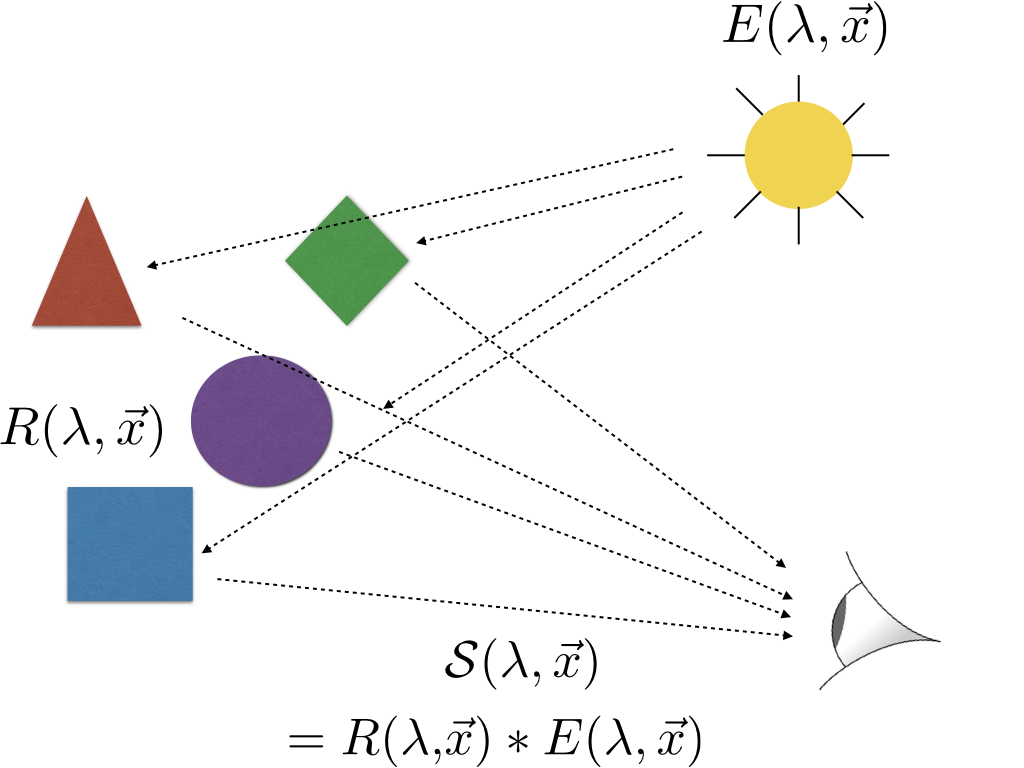
\includegraphics[width=\textwidth]{../Figures/Figure1/Figure1_a.png}
        \caption{}
        \label{fig:introSchematic}
    \end{subfigure}
    \begin{subfigure}{0.45 \textwidth}   
        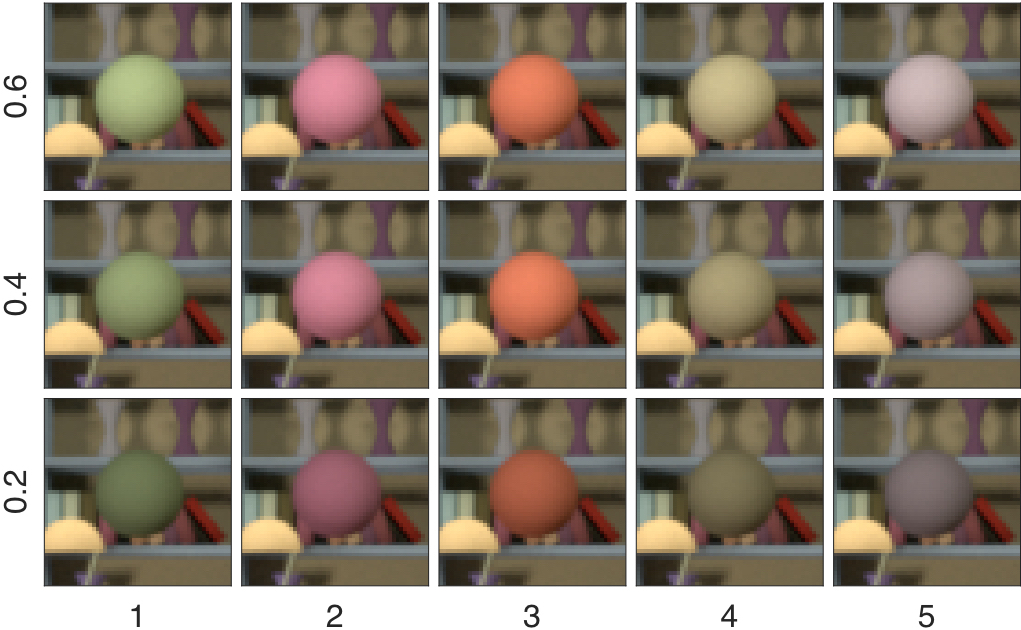
\includegraphics[width=\textwidth]{../Figures/Figure1/Figure1_b.jpeg}
        \caption{}
        \label{fig:introExampleFigure}
    \end{subfigure}
    \label{introFigure}
    \caption{(a) {\bf Color Constancy:} The light reflected off an object and incident on our eyes, depends both on the surface reflectance of the object $\left( R(\lambda,x) \right)$ and the illumination spectrum of the light source $\left(E(\lambda,x)\right)$. Additionally, the reflected light also depends on context the object lies in. Thus a variation in the reflected light can result from either a change in the object surface reflectance, or a change in the illumination spectrum of the light source, or change in the context, or all of these. Color constancy refers to the ability of the human visual system to perceive the color of the object stably under variations coming from these factors. (b) {\bf Lightness Constancy Under Spectral Variations:} In this work we study lightness constancy under variations in the spectra of the light sources and the objects. In Fig.\ref{fig:introExampleFigure}, we show 5 images generated at three different lightness levels of the target object (spherical object in the center). Along the rows we have fixed the lightness level of the target object, while we vary the spectra of the target object, the background objects and the light sources. (For illustration, in fig.\ref{fig:introExampleFigure}, We have fixed the shape of the target object reflectance spectra along the column.) Our aim is to identify computations that can recover the target object lightness from such stimuli.} 
\end{figure}

The variations in the reflected light can result from either geometrical factors (like shape, size, relative position of objects, etc.) or spectral factors (such as the illumination spectra, surface reflectance, diffusivity, etc.). In this work, we focus on the spectral factors. Specifically, we study the effects of variations in the surface reflectance spectra and the illumination spectra on lightness perception. We are interested in identifying the computations that can lead to stable lightness perception and constancy (Fig.\ref{fig:introExampleFigure}).

\begin{comment}
\begin{figure}
\centering
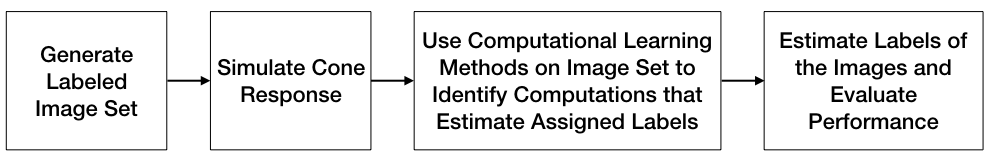
\includegraphics[width=\textwidth]{approach.png}
\caption{{\bf Approach:} We have employed a supervised learning approach to study color constancy. We first generate a large dataset of multi-spectral images labeled with the lightness level of the target object. We generate images at multiple lightness levels, with images at the same lightness level having variable object reflectance spectra and illumination spectra. These multi-spectral images are used to simulate the response of the visual system. We use isetbio toolbox to model the optics and physiology of early vision and produce the response of the cones in the retina. We use supervised computational learning methods on this labeled dataset of cone-responses to estimate the lightness of the target object. The performance of the supervised method is calculated using a separate test dataset.} 
\label{fig:approach}
\end{figure}
\end{comment}

We employ a supervised learning approach to understand this phenomenon. Our approach involves generating a database of multi-spectral images of naturalistic scenes. These images are labeled by the lightness of a specific target object in the scene. The image label depends on the reflectance of the target object. It refers to the perceived lightness of the target object if it were placed under a standard light source ($D_{65}$ daylight spectrum). We generate hundreds of multi-spectral images at several fixed values of the target object standard lightness. At a particular lightness level, we allow variations in the surface reflectance spectra of the objects (both the target and the surround objects) and the illumination spectra of the light sources (Fig. \ref{fig:introExampleFigure}. 

In this work, we study three cases resulting from the combination of such spectral variations (Fig.\ref{fig:studiedCases}. These cases are: 1. Variations in target object spectra (Fig.\ref{fig:targetVarying}) with fixed illumination and background surface reflectance spectra, 2. Variations in target object spectra and the light source spectra, with fixed background surface reflectance spectra (Fig.\ref{fig:targetIlluminantVarying}), and 3. Variations in all spectra (target object, background object and light source) (Fig.\ref{fig:allSpectraVarying}). The effects of other types of spectral variations can be explained in terms of one of these cases (see supplementary information).

% Figure 2: Cases Studied
\begin{figure}
\centering
	\begin{subfigure}[b]{0.33 \textwidth}
		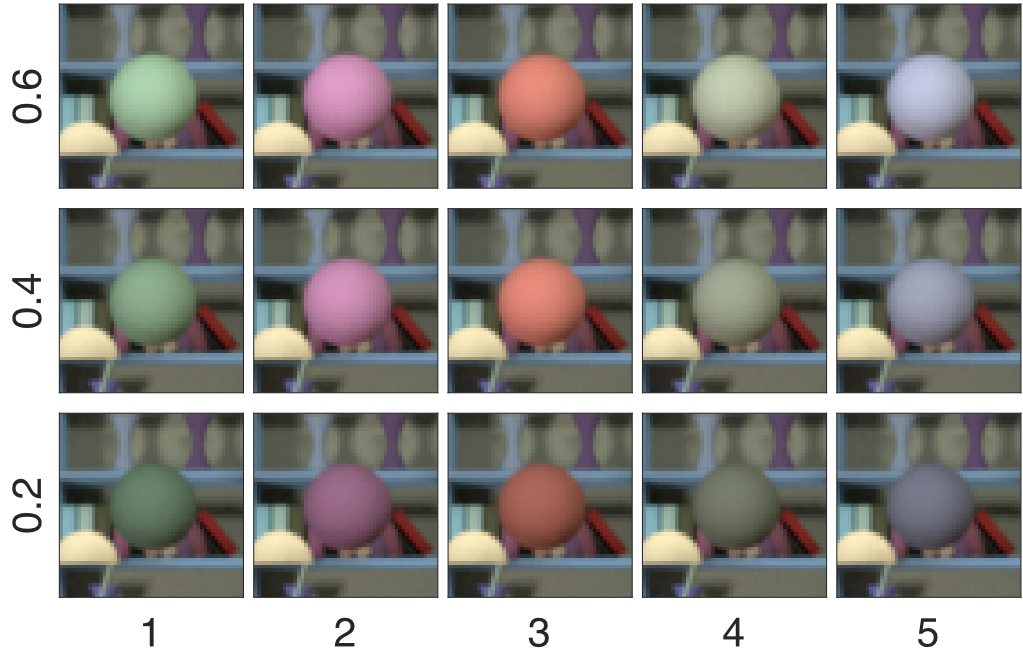
\includegraphics[width=\textwidth]{../Figures/Figure2/Figure2_a.jpeg}
		\caption{Case 1}
 		\label{fig:targetVarying}
	\end{subfigure}
	\begin{subfigure}[b]{0.33 \textwidth}
        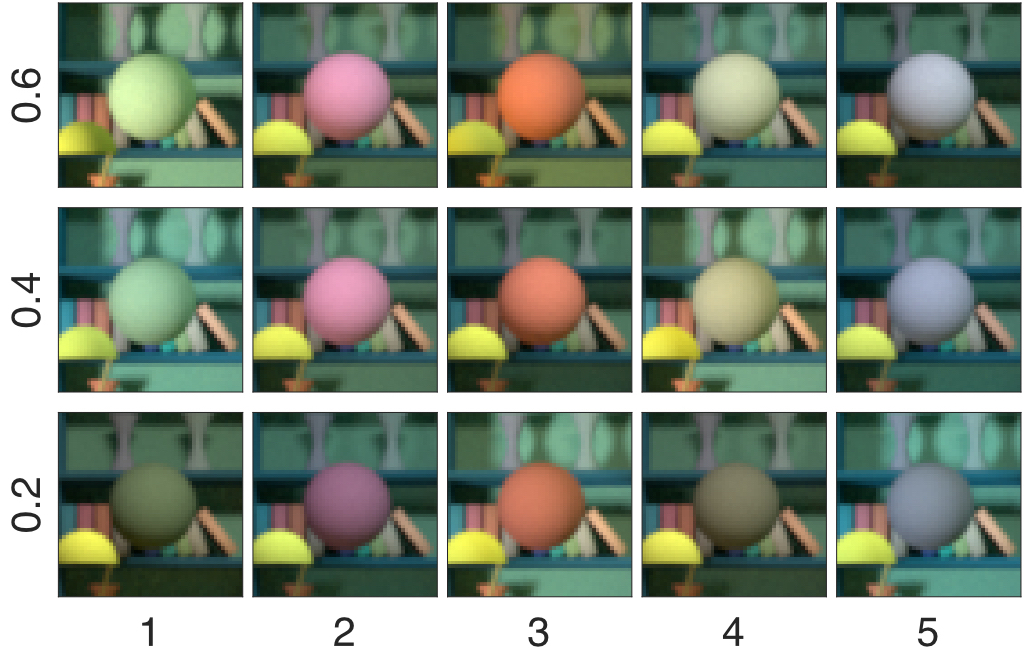
\includegraphics[width=\textwidth]{../Figures/Figure2/Figure2_b.jpeg}
        \caption{Case 2}
        \label{fig:targetIlluminantVarying}
    \end{subfigure}
	\begin{subfigure}[b]{0.33 \textwidth}
        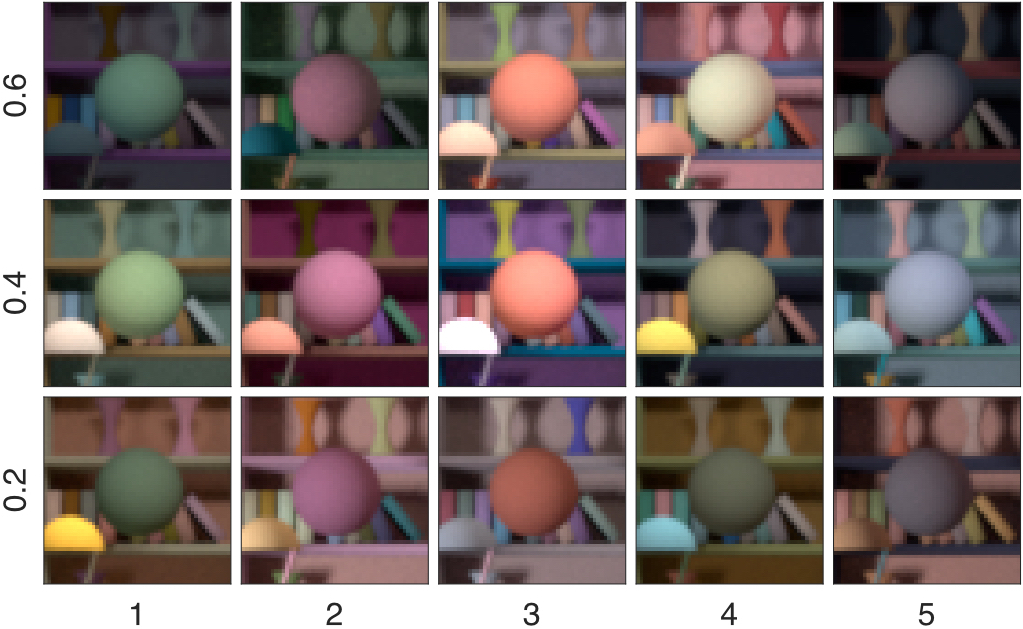
\includegraphics[width=\textwidth]{../Figures/Figure2/Figure2_c.jpeg}
        \caption{Case 3}
        \label{fig:allSpectraVarying}
    \end{subfigure}    
    \caption{{\bf Three types of spectral variations studied in this work:} sRGB rendition of images studied in our work. The numbers on the left are the standard lightness level of the target object. We show 5 images for each case at 3 lightness levels. The analysis was performed with images at 10 lightness levels. We studied three types of spectral variations. (a) Case 1: Target reflectance spectra variable, Background reflectance spectra fixed, illuminant spectra fixed (b) Case 2: Target reflectance spectra variable, Background reflectance spectra fixed, illuminant spectra variable (c) Case 3: Target reflectance spectra variable, Background reflectance spectra variable, illuminant spectra variable.}
\label{fig:studiedCases}
\end{figure}

After generating databases of labeled multi-spectral images for each one of these cases, we simulate the response of the cones in the retina cone using an accurate model of the eye. These cone-responses datasets, that are labeled with the standard lightness of the target object, are then analyzed using supervised computational learning methods. 

We have employed three supervised computational learning methods for estimating the target object lightness: linear regression, a generalized SVD regression and accuracy maximization analysis (AMA). The linear regression has been performed on the cones corresponding to the center pixel of the target object. The other two methods take the response of all the cones in the model retina. While, SVD regression a linear transformation to estimate the lightness, AMA uses a non-linear transform of the data. These methods identify the computations that need to be performed on the cone-responses to estimate the target object lightness. Finally, we evaluate the performance of the computational methods on a test set of images.

In the following, we describe each one of these stages of our approach in detail. In the methods section, we first describe the process to generate naturalistic labeled images (\nameref{method:VirtualWorld}). Next, we describe the steps to simulate the response of the retinal cones to these images (\nameref{method:Isetbio}). Finally, we describe the three learning methods we have used in our analysis (\nameref{method:SupervisedLearning}). In the results section, we show the estimates and performance of each one of the supervised methods for the three cases with different spectral variations. 

We show that for spectral variations that allow variation either only in the target surface reflectance or the background surface reflectance or the spectral power distribution of the source of light, the standard lightness, $Y_{65}$ can be recovered by simple manipulations of the reflected light captured by the visual system. For example, if the illumination spectra of the light sources and the background are held fixed, while the target reflectance spectra change (case 1), $Y_{65}$ can be recovered directly from the light reflected off the target object. If the surface reflectance of the target object and the illumination spectra of the light sources are allowed to vary, but the background reflectance spectra is fixed (case 2), $Y_{65}$ can be recovered by from the contrast between the target and the background. When all the spectral features in the scene are allowed to change (case 3), $Y_{65}$ can not be recovered from a simple manipulations of the light captured by the visual system. Here, we have used a Bayesian supervised learning method called accuracy maximization analysis to estimate $Y_{65}$ of the target object. Using this method, we can recover the lightness of the target object with $\sim 15\%$ relative root mean square error.

Finally, we compared the generality of the methods for lightness estimation by comparing the optimal receptive fields of one case to the others. The optimal receptive fields for estimating the lightness of the target object show a center surround structure, supporting a comparison between the light coming from the target object and its surround. Additionally, the receptive fields give more weight to the L and M cone responses compared to S cone responses. We discuss the implications of such receptive fields on lightness constancy. 

\section{Methods}
\subsection{Image database} \label{method:VirtualWorld}
In this section we briefly describe our image generation software, that we call Virtual world color constancy (VWCC). The details of the software are provided in the supplementary information section. To generate a virtual scene, we first select a 3D scene, a target object and a light source from the set of predefined scenes and objects of the VWCC software. The target object and the light source are inserted at predefined positions in the 3D scene. Fig.\ref{fig:3DScene} shows a 2D sRGB rendition of the 3D scene with the inserted target object (green sphere in the middle) used in our analysis. (The light source in not visible.) Next, we assign a surface reflectance spectrum and an illumination spectrum to each object and light source in the scene. The surface reflectance of the target object is assigned such that the perceived lightness of the target object under D65 daylight spectrum has a fixed value. Once these spectral properties have been assigned, we render a 320x240 pixel$^2$ 2d multi-spectral images of the scene at 31 frequencies (linearly spaced between 400nm - 700nm) using a graphics rendering system called Mitsuba \cite{jakob2015mitsuba}. We generate hundreds of such scenes and corresponding multi-spectral images for at 10 linearly spaced lightness levels between 0.2 and 0.6. For the images at a fixed lightness level, the reflectance and illumination spectra are assigned according to the spectral variations allowed under each case. Next, we crop a 51x51 pixel$^2$ part of the multi-spectral image containing the target object for further analysis (\ref{fig:croppedImage}). Fig. \ref{fig:studiedCases} shows examples of such cropped image at 3 lightness levels for the three cases considered in this work.

% Figure 3: Methods
\begin{figure}
\centering
\begin{subfigure}[b]{0.25 \textwidth}
		\centering
        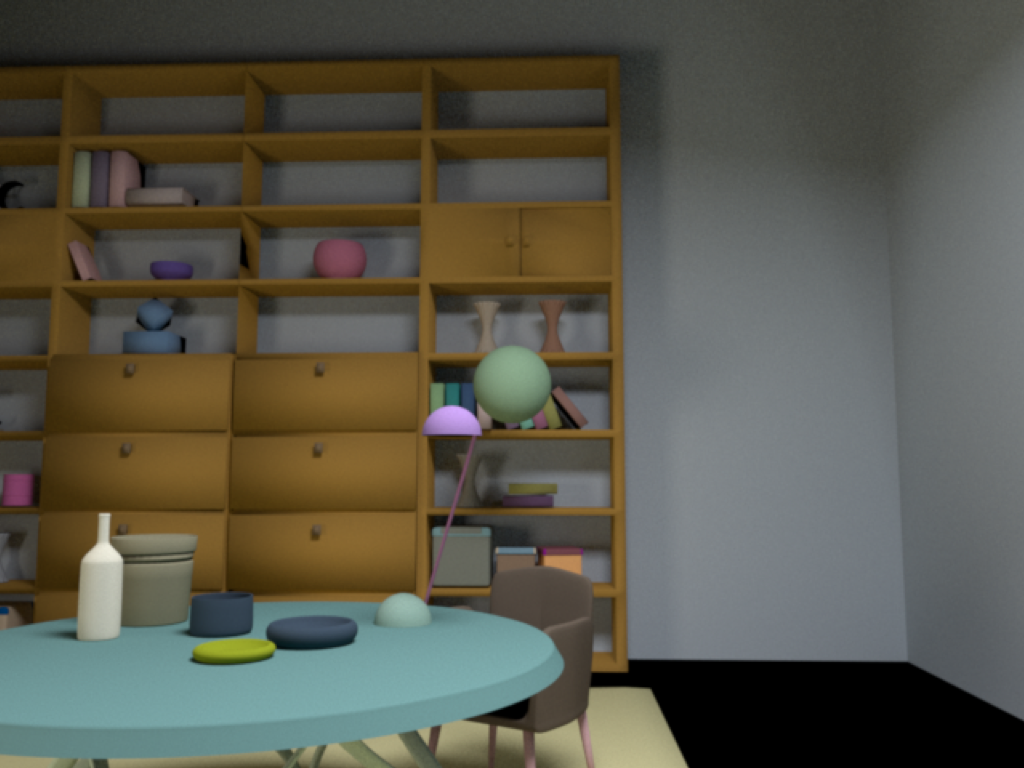
\includegraphics[width=\textwidth]{../Figures/Figure3/Figure3_a.png}
        \caption{A typical 3D Scene}
        \label{fig:3DScene}
    \end{subfigure}
    ~ %add desired spacing between images, e. g. ~, \quad, \qquad, \hfill etc. 
      %(or a blank line to force the subfigure onto a new line)
    \begin{subfigure}[b]{0.19 \textwidth}   
    \hspace{0.1 \textwidth}
        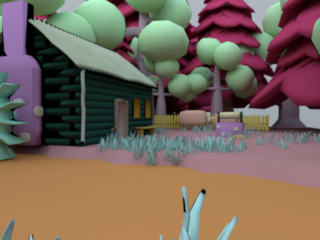
\includegraphics[width=\textwidth]{../Figures/Figure3/Figure3_b.png}
        \caption{Cropped Image}
        \label{fig:croppedImage}
    \end{subfigure}
    ~ %add desired spacing between images, e. g. ~, \quad, \qquad, \hfill etc. 
    %(or a blank line to force the subfigure onto a new line)
    \begin{subfigure}[b]{0.19 \textwidth}
    \hspace{0.1 \textwidth}
        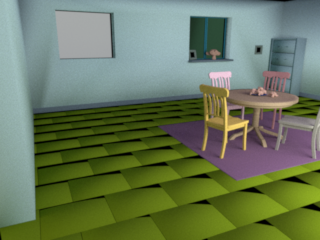
\includegraphics[width=\textwidth]{../Figures/Figure3/Figure3_c.png}
        \caption{Optical Image}
        \label{fig:croppedImageWithMosaic}
    \end{subfigure}
    ~
    \begin{subfigure}[b]{0.2 \textwidth}
        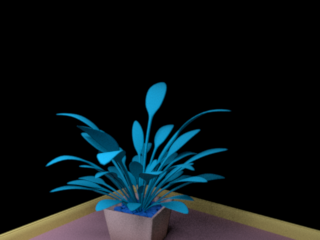
\includegraphics[width=\textwidth]{../Figures/Figure3/Figure3_d.png}
        \caption{LMS cone contrast}
        \label{fig:coneContrast}
    \end{subfigure}

    \label{fig:sceneWithCroppedImage}
    \caption{{\bf Generating labeled dataset for computational analysis:}  We employ a supervised learning approach in our study. We generate a database of visual system response to images labeled with the lightness of the target object. This is done as follows: (a) We define a 3D virtual scene where we can assign the geometrical and spectral properties of the objects. In this 3D scene, we place a target object (here the spherical object) in the camera field of view and assign a fixed reflectance spectrum to the target object. Then we render a hyperspectral image of the scene. (b) A part of the image, containing the target object, is cropped from the image. (c) Using an accurate model of the front end of the visual system, we generate the response of the retinal cones to the cropped image. Fig.\ref{fig:croppedImageWithMosaic} shows the optical image incident on the cone mosaic and the location and the identity of the cones (L cones: Red, M cones: Green, S cones: Blue). See text for the details of the model. (d) For each cone type, we interpolate the response to get the cone-response of all the three types at each location. These responses are contrast normalized (see text) to the get the input analysis.}
\end{figure}

\subsection{Model of Visual System} \label{method:Isetbio}
We simulate the visual system response using isetbio software toolbox. Isetbio simulates a model of the visual system accounting for cornea, pupil size, lens and physiological optics. We use the multi-spectral cropped image (fig.\ref{fig:croppedImage}) as the optical stimulus to simulate the response of the cones in the retina. The cropped image patch is assumed to cover a $1^{\circ}$ field of view at a distance of 1 m. The retinal cone mosaic is modeled as a square grid with 51x51 cones in the l:m:s ratio 0.6:0.3:0.1. The response of the cones are measured in terms of the number of isomerizations in the cone segment ({\it over what time ??}). Since, S cones response are much lower than of L and M cones, to model the amplification of the S cone response downstream, we rescale the cone response functions by the total area under the response curves. This leads to comparable number of isomerizations in the L, M and S cone on the presentation of an image. We interpolate the responses of cones in each cone class to get a $51 \times 51$ cone response image for each cone class.  

The three $51 \times 51$ cone response matrix corresponding to each one of the L, M and S cones are then reshaped into a $7803 \times 1$ vector. To model the contrast adaptation in the visual system, we subtract the mean of the vector from each entry and divide by the mean. We further rescale the vector to have norm 1. The cone-response vectors corresponding to the N images for each case are concatenated into a $7803 \times N$ contrast normalized matrix $C$. The corresponding labels are represented by a $1 \times N$ row vector $Y$.

\subsection{Supervised Learning methods} \label{method:SupervisedLearning}
\subsubsection*{Linear Regression} To estimate the target object lightness using linear regression, we solve the equation $A_{(1,3)}*C_{(3,N)} = Y_{(1,N)}$. Here, $Y_{(1,N)}$ corresponds to the row vector of the lightness labels for the N images in the dataset. $C_{(3,N)}$ corresponds to the matrix of cone responses corresponding to the central pixel. Each column represents the response to one image and the rows corresponds to the contrast normalized L, M and S cone response of the center pixel. The coefficient matrix $A$ can be obtained as $A = Y*C^{-1}$. 

The L, M and S response to the center pixel on the target object is calculate by taking the average of a 3x3 patch of cones near the center of the target.

\subsubsection*{SVD regression}
This 
\subsubsection*{Accuracy maximization analysis}

\subsection{Types of spectral variations studied}
In this work we have studied the effects of spectral variations on perceived lightness. The spectral variations in the scene can be categorized into three types. The variations in the shape of target object reflectance spectra, the variations in the shape of background object reflectance spectra, and the variations in the shape of the spectral power distribution of light sources. Here, we present the results for three cases (fig.\ref{fig:studiedCases}): 1. effects of variations in target object spectra (fig.\ref{fig:targetVarying}), 2. effects of variations in target object spectra and the light source spectra (fig.\ref{fig:targetIlluminantVarying}), and 3. effects of variations in all three spectra (fig.\ref{fig:allSpectraVarying}). The rest of the cases are qualitatively similar to one of the cases discussed here, and are discussed in the supplementary materials. 


\section{Results}
\subsection{Case 1}

% Figure 4
\begin{figure}
\centering
\begin{subfigure}[b]{0.27 \textwidth}
		\centering
        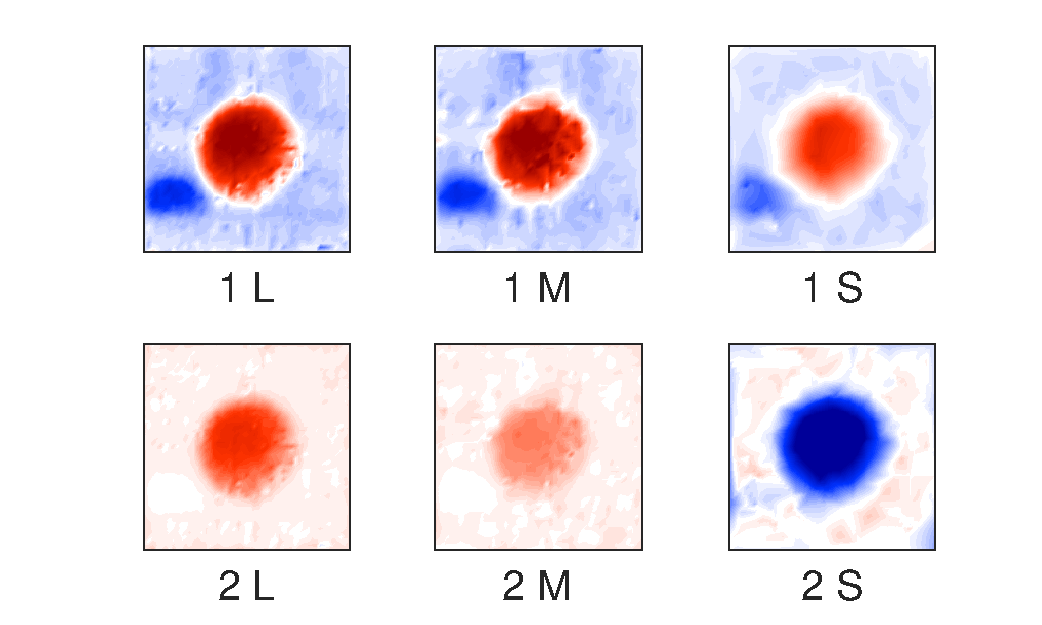
\includegraphics[width=\textwidth]{../Figures/Figure4/Figure4_a.pdf}
        \caption{SVD First 2 RFs}
        \label{fig:case9SVD}
    \end{subfigure}
    \begin{subfigure}[b]{0.27 \textwidth}   
        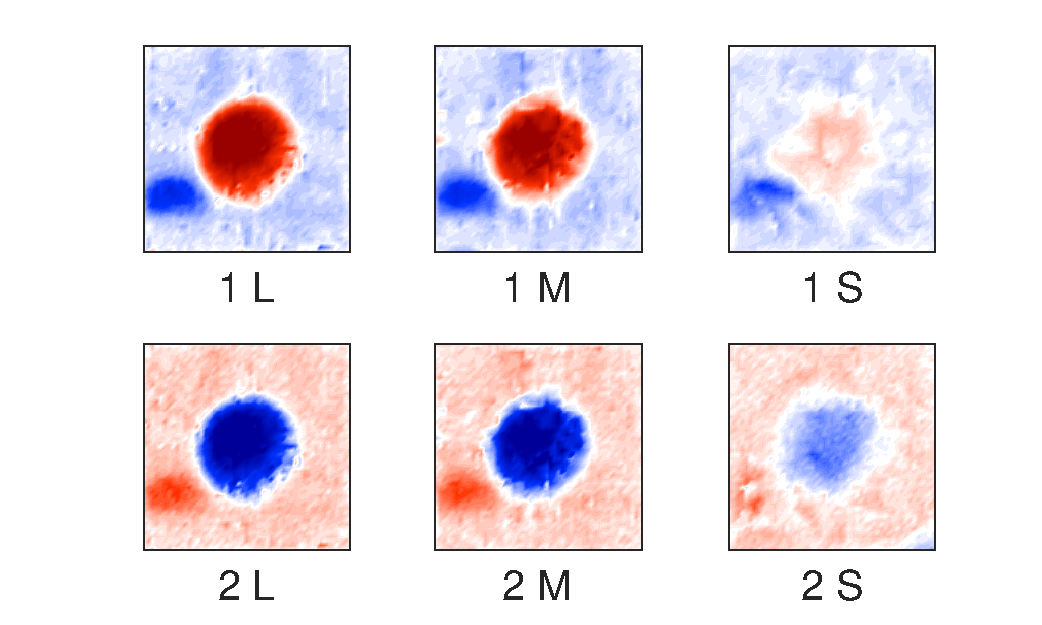
\includegraphics[width=\textwidth]{../Figures/Figure4/Figure4_b.pdf}
        \caption{AMA First 2 RFs}
        \label{fig:case9AMA}
    \end{subfigure}
        \begin{subfigure}[b]{0.20 \textwidth}
        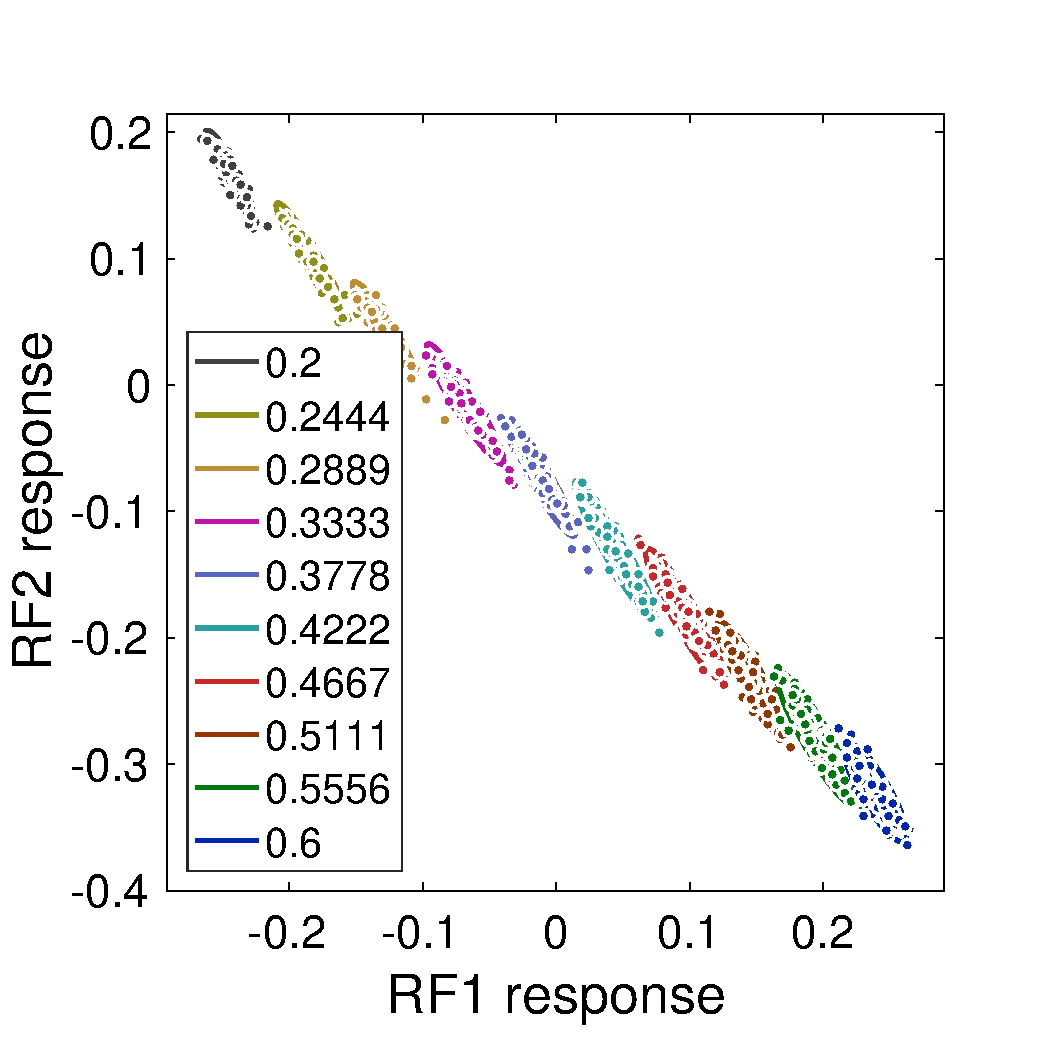
\includegraphics[width=\textwidth]{../Figures/Figure4/Figure4_c.pdf}
        \caption{AMA RF Response}
        \label{fig:case9FiltersResponse}
    \end{subfigure}
        \begin{subfigure}[b]{0.20 \textwidth}
        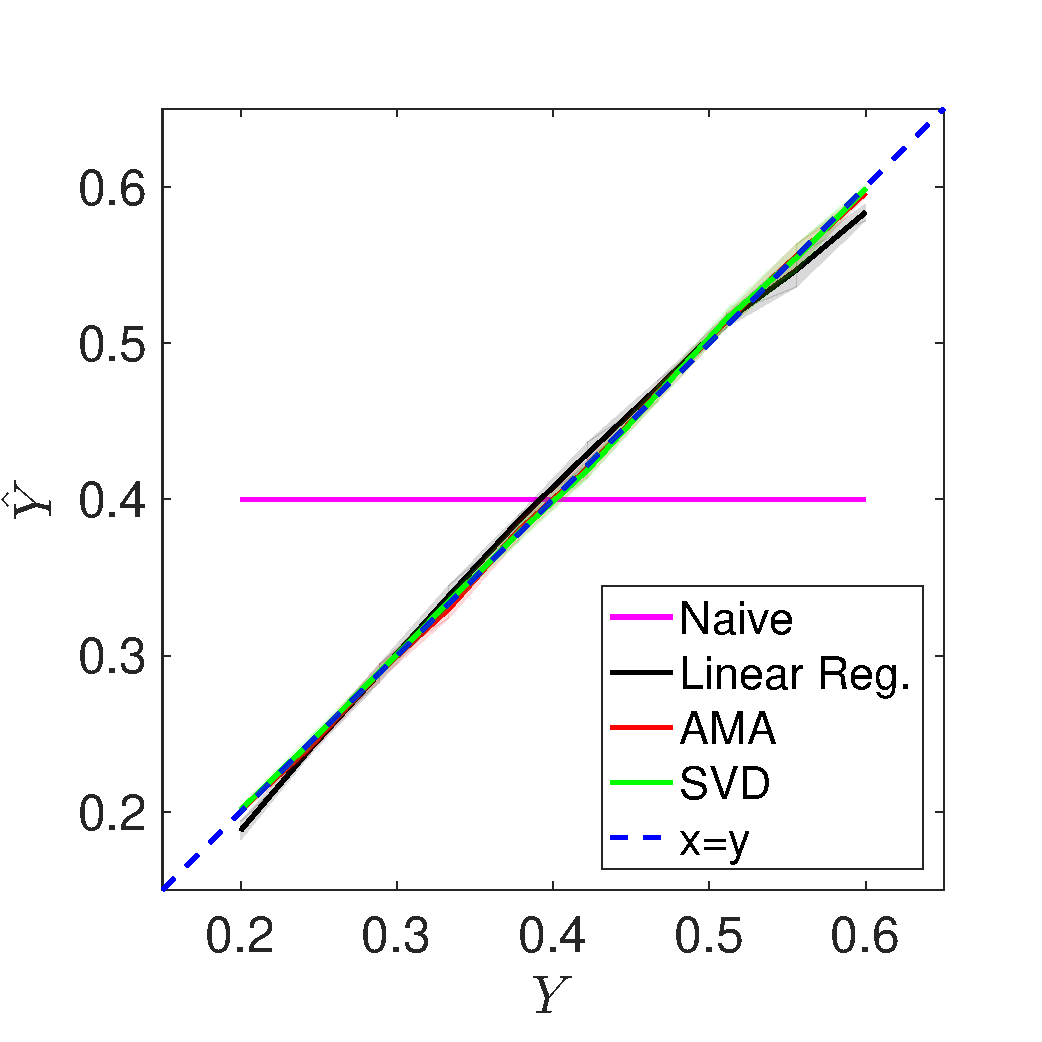
\includegraphics[width=\textwidth]{../Figures/Figure4/Figure4_d.pdf}
        \caption{Lightness Estimates}
        \label{fig:case9Results}
    \end{subfigure}    
    \caption{{\bf Receptive fields and lightness estimates. Case 1:} (a) First two receptive fields produced by the SVD method. Along the row we show the filters corresponding to the L cones, M cones and Scones (left to right). (c) First two receptive fields produced by the SVD method. (c) The response of the stimuli to the first two AMA filters. The responses are grouped with the label of the stimuli. As is clear, the response separate out quite well in this case, making the estimation easy (d) The estimates of the target object standard lightness. The naive method produces the mean value of the target luminance used in the analysis. The shaded region corresponds to 1 sigma standard deviation.}
\label{fig:case9AllResults}
\end{figure}

% Figure 5
\begin{figure}
\centering
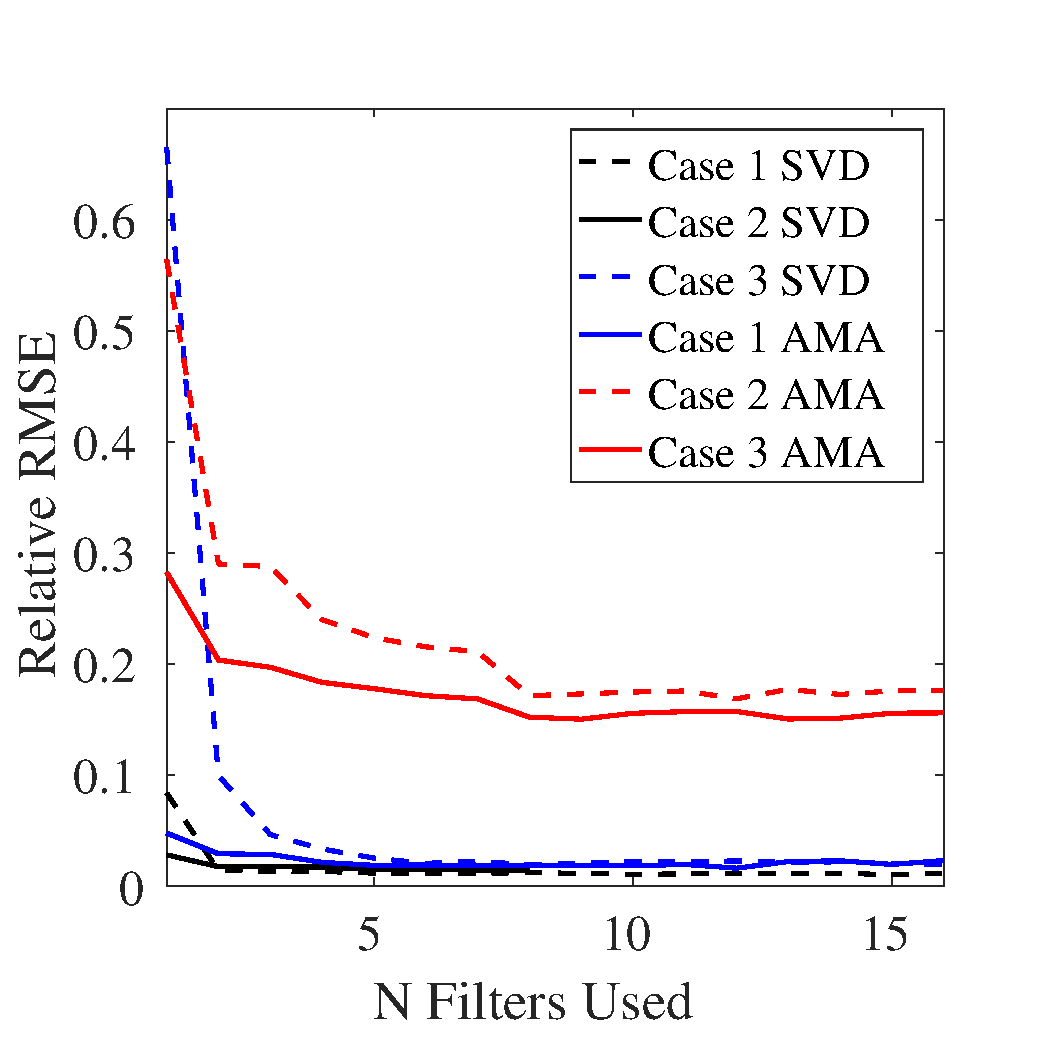
\includegraphics[width=0.3\textwidth]{../Figures/Figure5/Figure5.pdf}
\caption{{\bf Performance with number of RFs used for estimation:} Most of the information is captured by the first two filters. We have used the first 8 RFs in our analysis.}
\label{fig:RMSEvsNFilters}
\end{figure}

% Figure 6
\begin{figure}
\centering
\begin{subfigure}[b]{0.27 \textwidth}
		\centering
        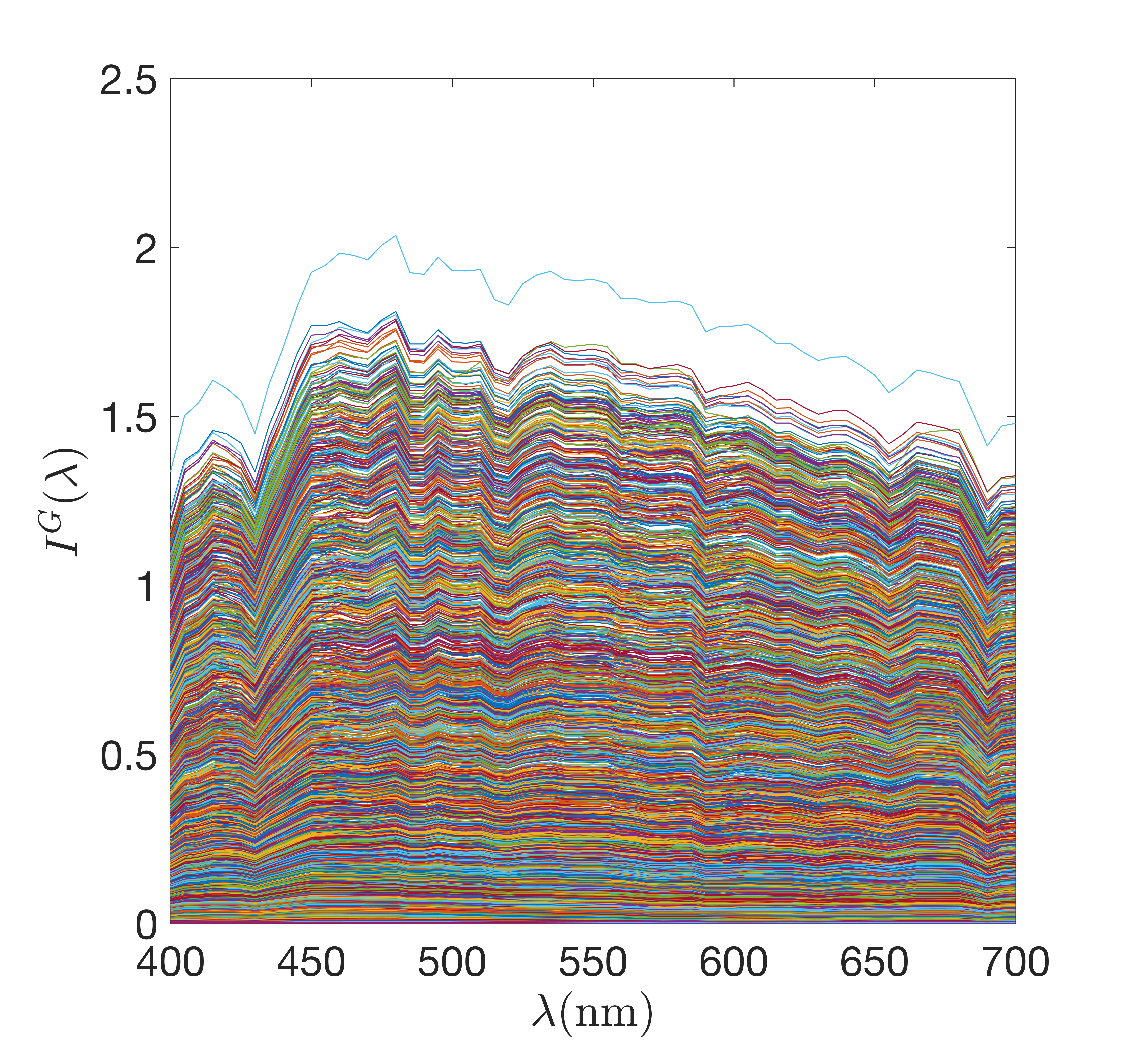
\includegraphics[width=\textwidth]{../Figures/Figure6/Figure6_a.pdf}
        \caption{SVD First 2 RFs}
        \label{fig:case10SVD}
    \end{subfigure}
    \begin{subfigure}[b]{0.27 \textwidth}   
        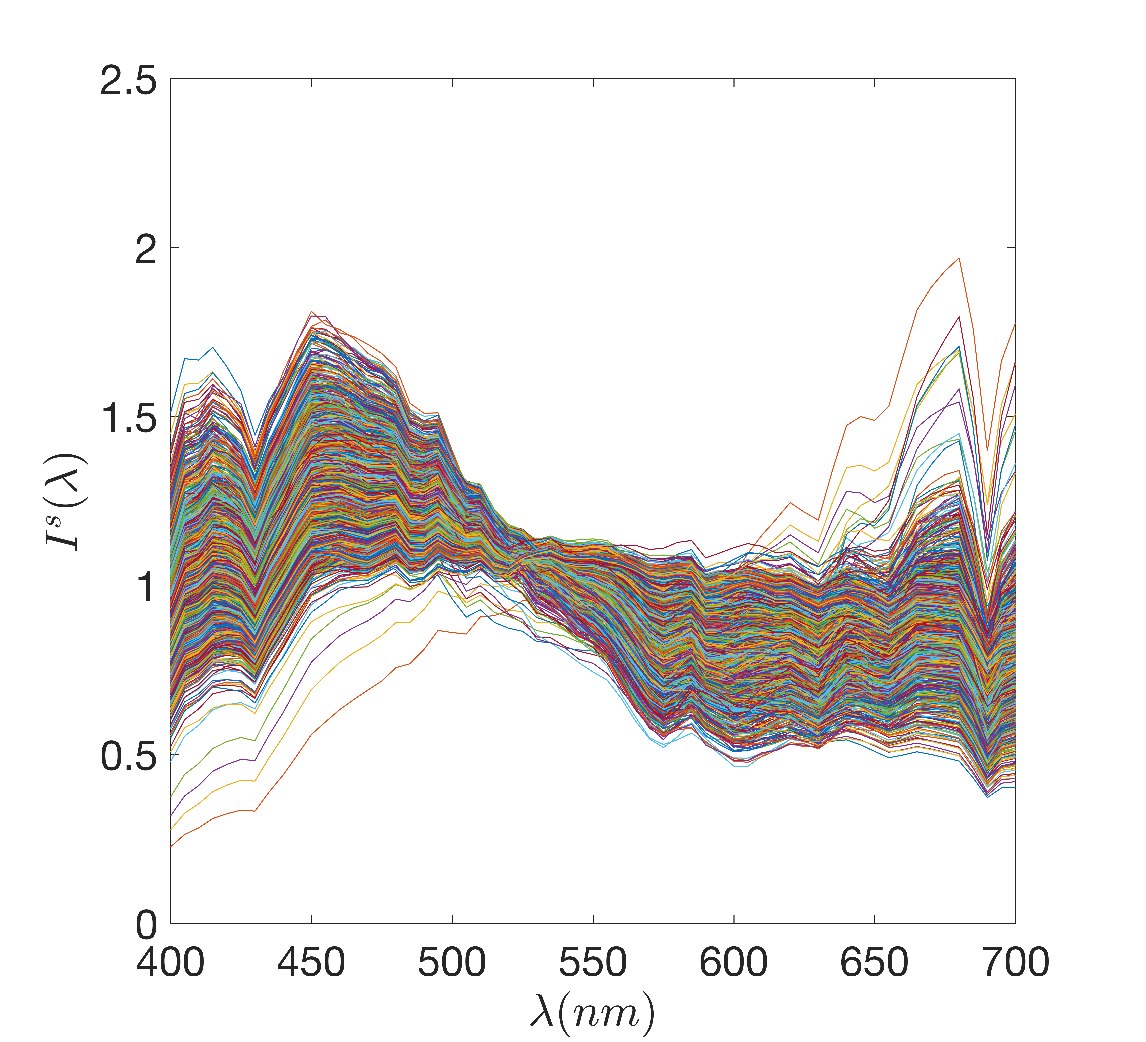
\includegraphics[width=\textwidth]{../Figures/Figure6/Figure6_b.pdf}
        \caption{AMA First 2 RFs}
        \label{fig:case10AMA}
    \end{subfigure}
        \begin{subfigure}[b]{0.20 \textwidth}
        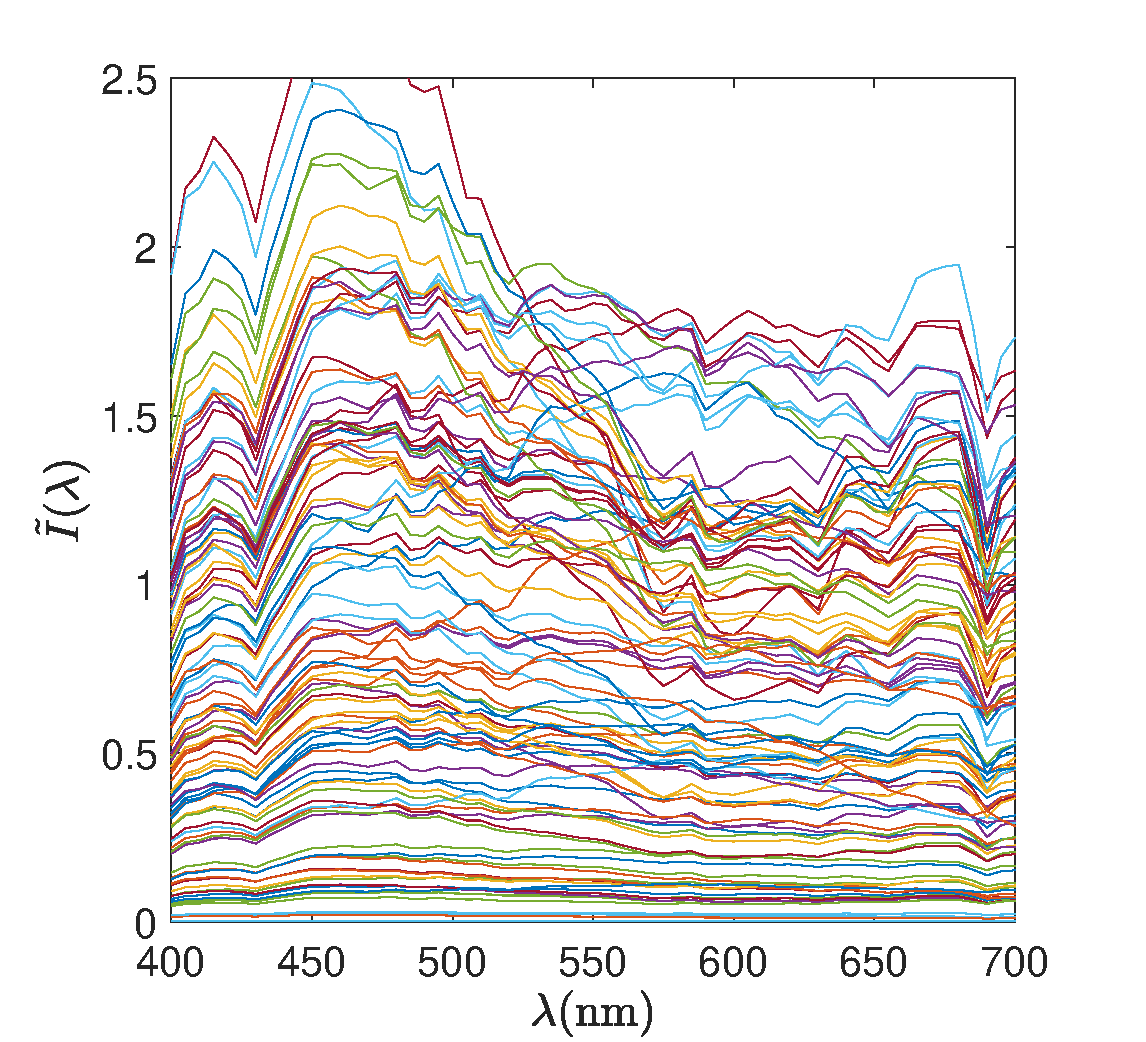
\includegraphics[width=\textwidth]{../Figures/Figure6/Figure6_c.pdf}
        \caption{AMA RF Response}
        \label{fig:case10FiltersResponse}
    \end{subfigure}    
        \begin{subfigure}[b]{0.2 \textwidth}
        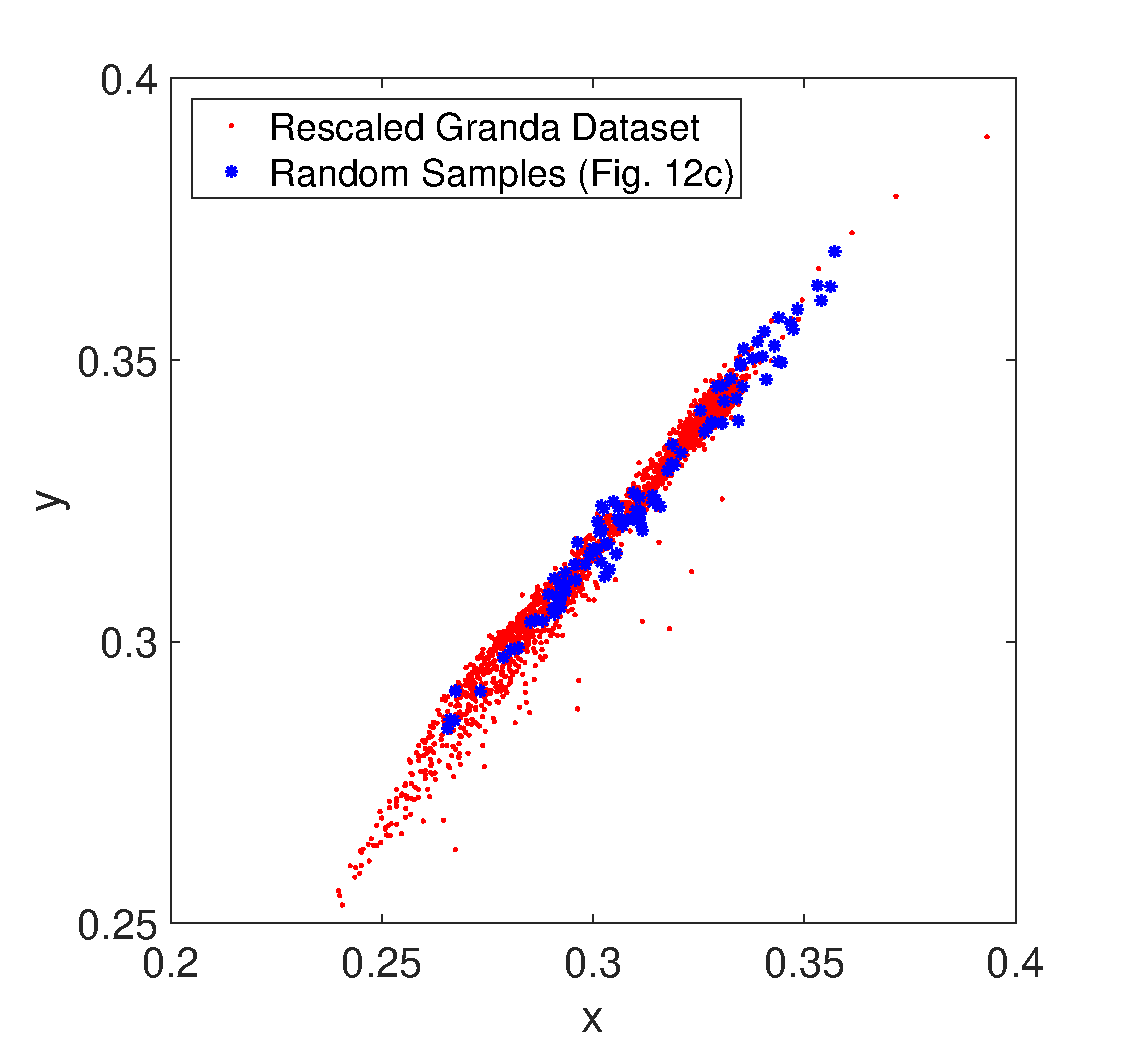
\includegraphics[width=\textwidth]{../Figures/Figure6/Figure6_d.pdf}
        \caption{Luminance Estimates}
        \label{fig:case10Results}
    \end{subfigure}
    \label{fig:case10AllResults}
    \caption{{\bf Receptive fields and lightness estimates. Case 2:} Same as Fig. \ref{fig:case9AllResults}.}
\end{figure}

% Figure 7
\begin{figure}
\centering
\begin{subfigure}[b]{0.27 \textwidth}
		\centering
        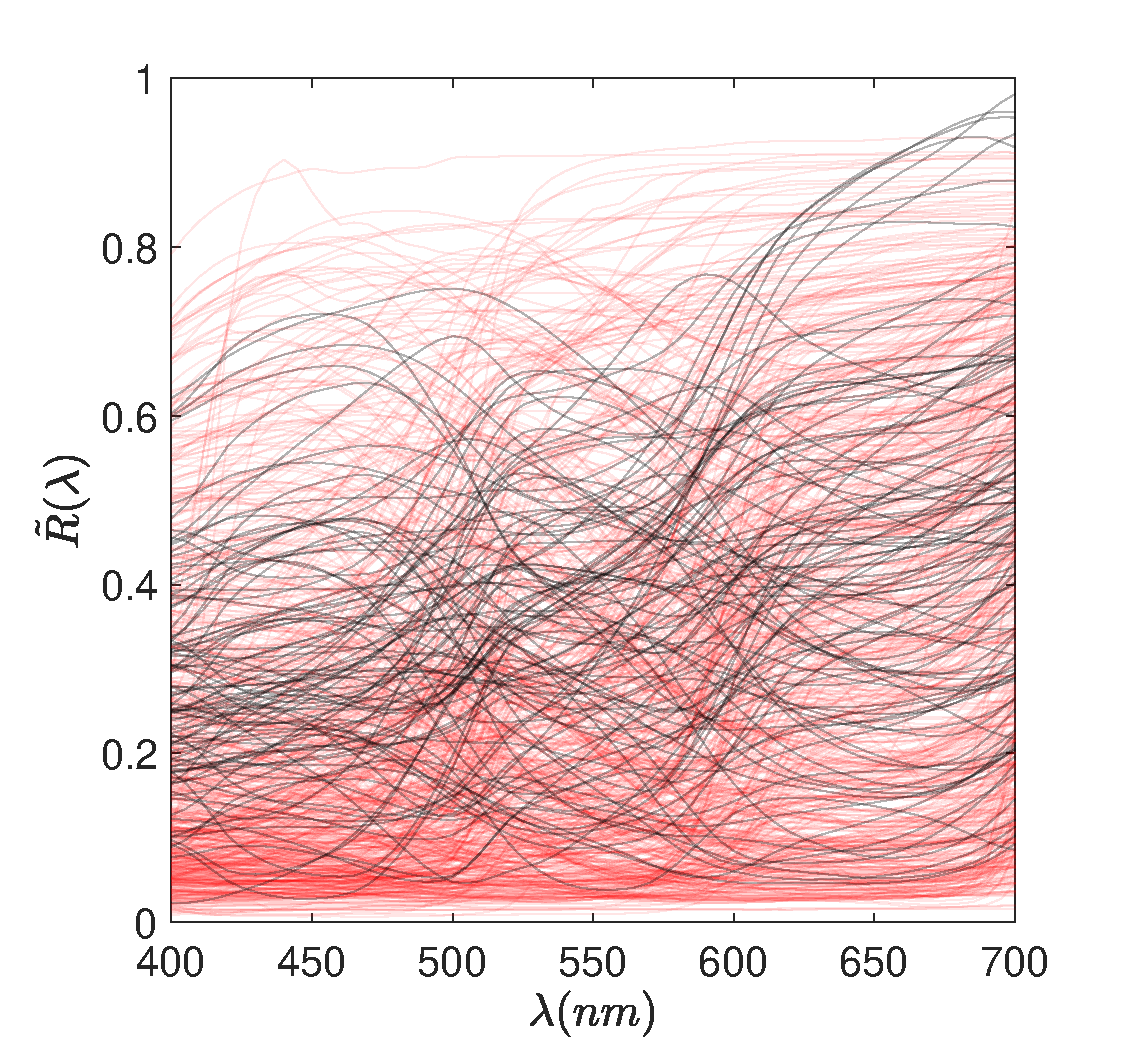
\includegraphics[width=\textwidth]{../Figures/Figure7/Figure7_a.pdf}
        \caption{SVD First 2 RFs}
        \label{fig:case12SVD}
    \end{subfigure}
    \begin{subfigure}[b]{0.27 \textwidth}   
        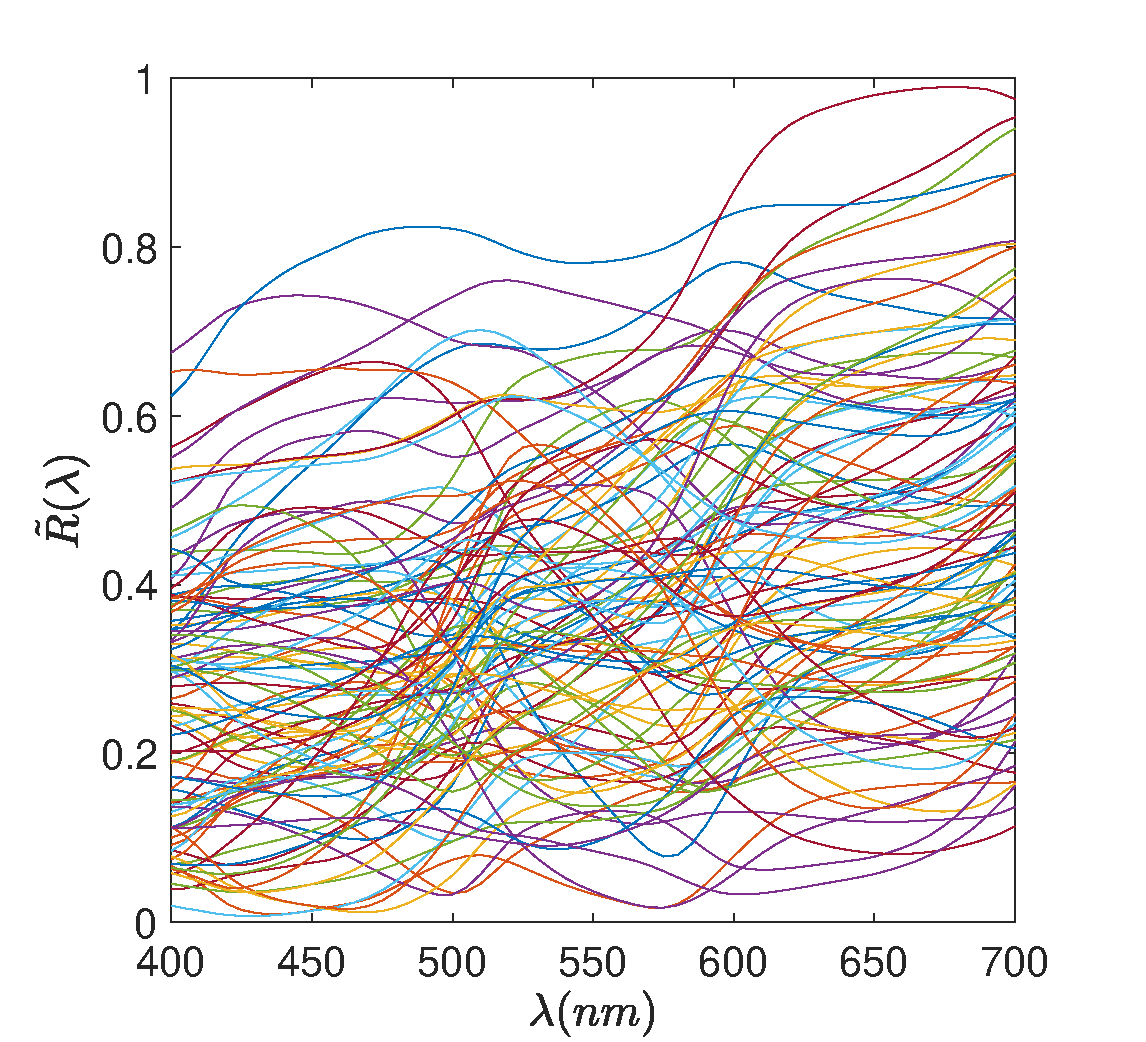
\includegraphics[width=\textwidth]{../Figures/Figure7/Figure7_b.pdf}
        \caption{AMA First 2 RFs}
        \label{fig:case12AMA}
    \end{subfigure}
        \begin{subfigure}[b]{0.20 \textwidth}
        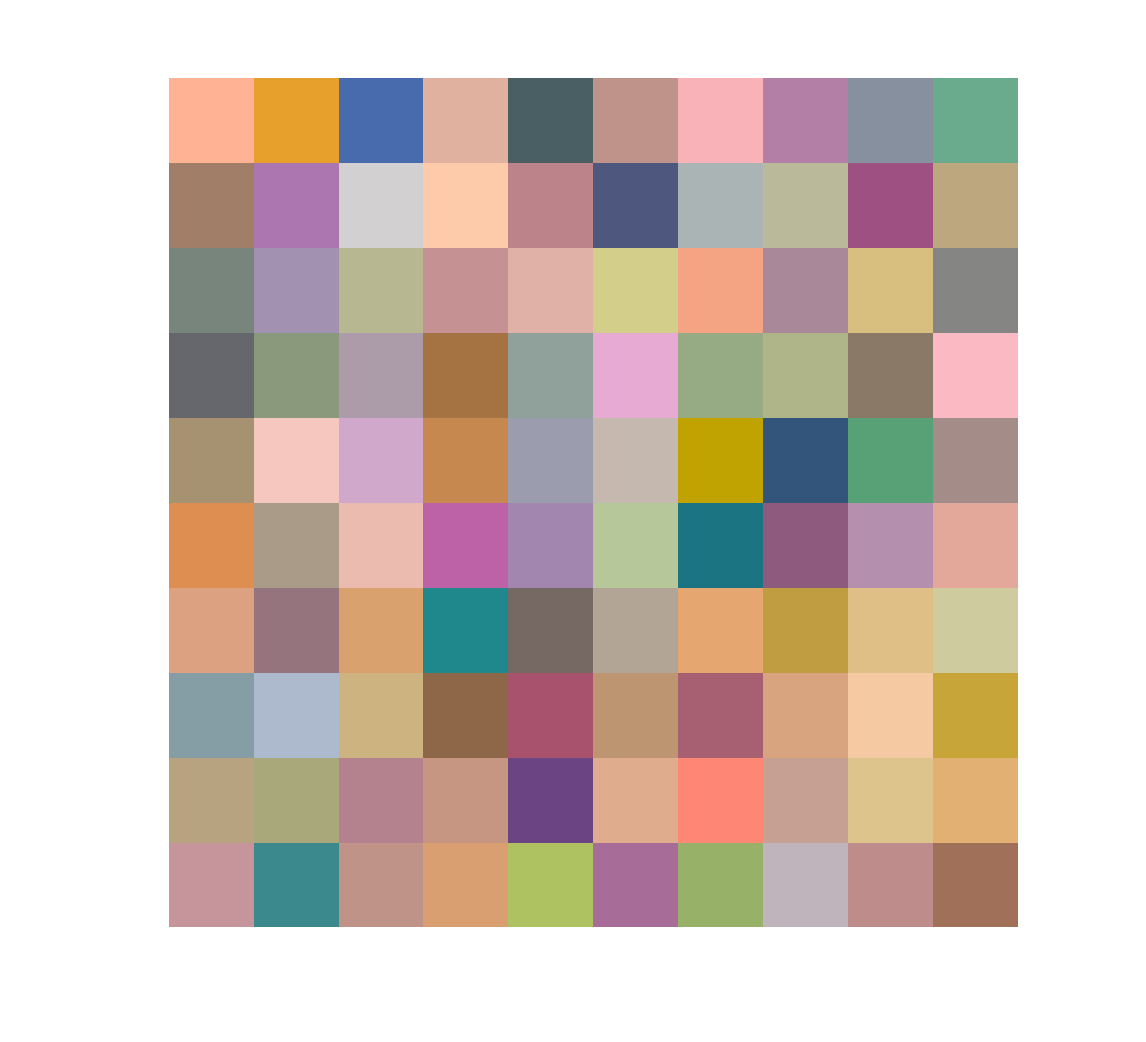
\includegraphics[width=\textwidth]{../Figures/Figure7/Figure7_c.pdf}
        \caption{AMA RF Response}
        \label{fig:case12FiltersResponse}
    \end{subfigure}    
        \begin{subfigure}[b]{0.2 \textwidth}
        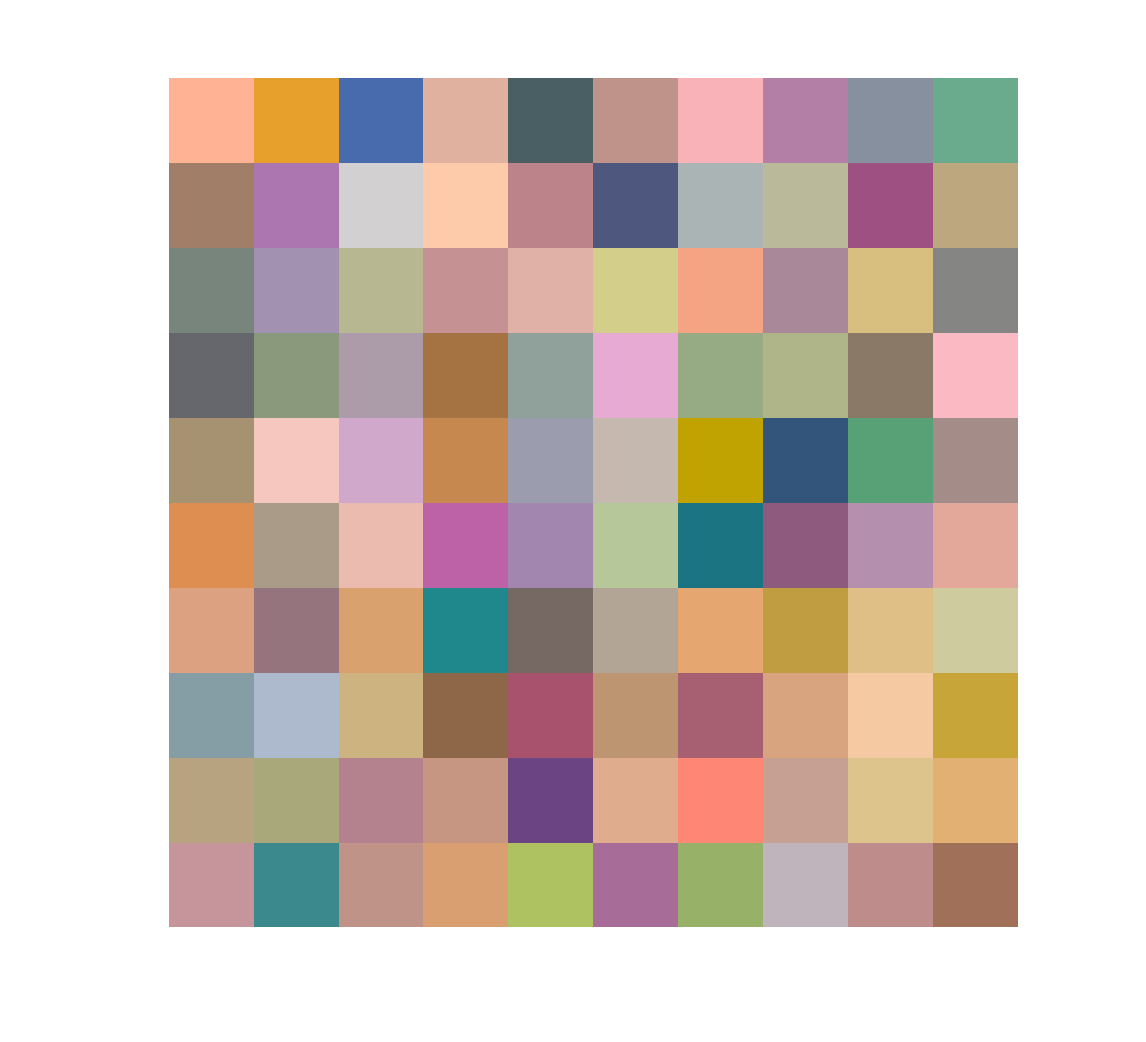
\includegraphics[width=\textwidth]{../Figures/Figure7/Figure7_d.pdf}
        \caption{Luminance Estimates}
        \label{fig:case12Results}
    \end{subfigure}
    \label{fig:case12AllResults}
    \caption{{\bf Receptive fields and lightness estimates. Case 3:}  Same as Fig. \ref{fig:case9AllResults}.}
\end{figure}

% Figure 8
\begin{figure}
\centering
\begin{subfigure}[b]{0.3 \textwidth}
	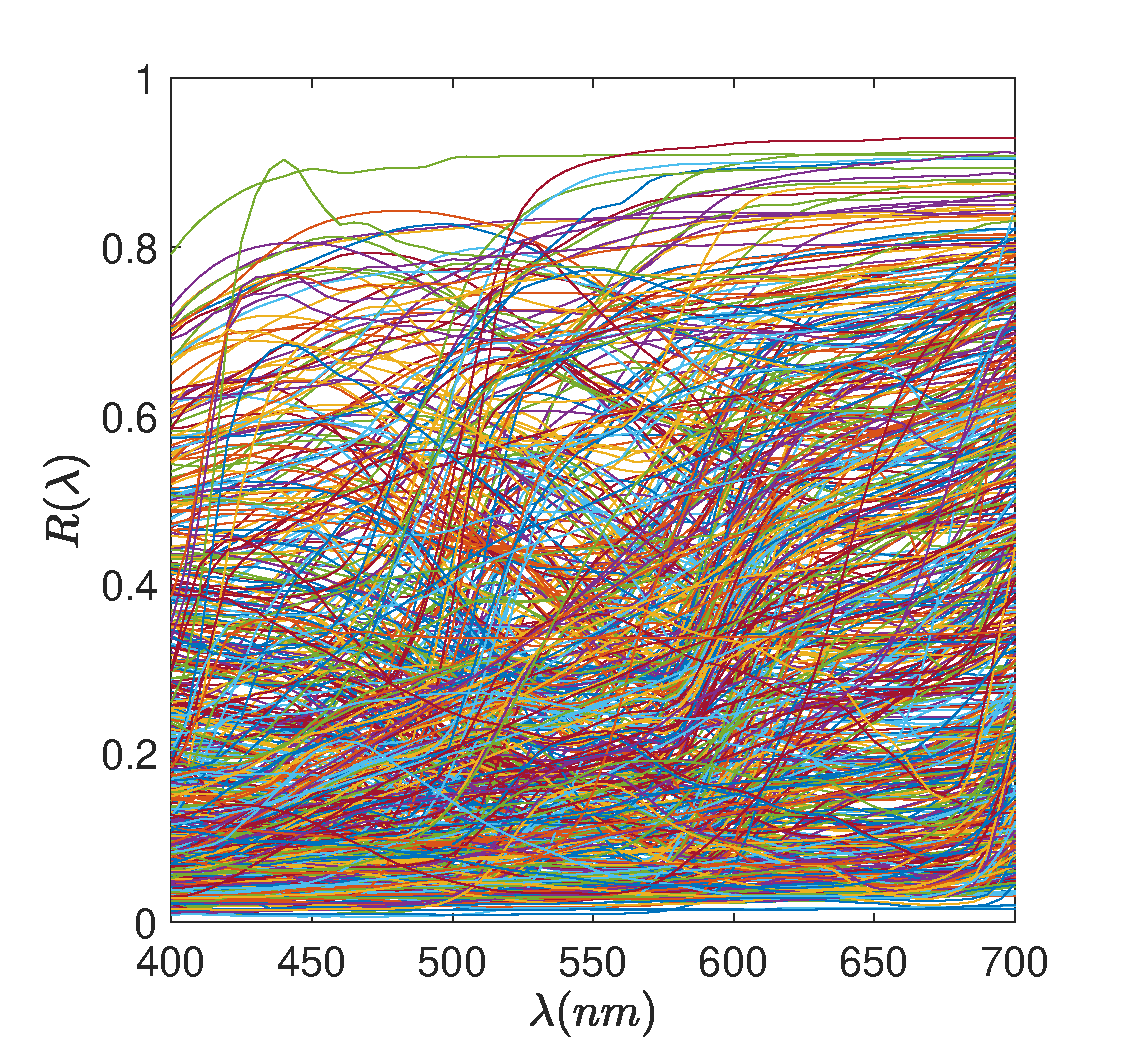
\includegraphics[width=\textwidth]{../Figures/Figure8/Figure8_a.pdf}
	\caption{Performance of methods}
	\label{fig:summaryBarGraph}
    \end{subfigure}
    ~ %add desired spacing between images, e. g. ~, \quad, \qquad, \hfill etc. 
      %(or a blank line to force the subfigure onto a new line)
    \begin{subfigure}[b]{0.3 \textwidth}   
	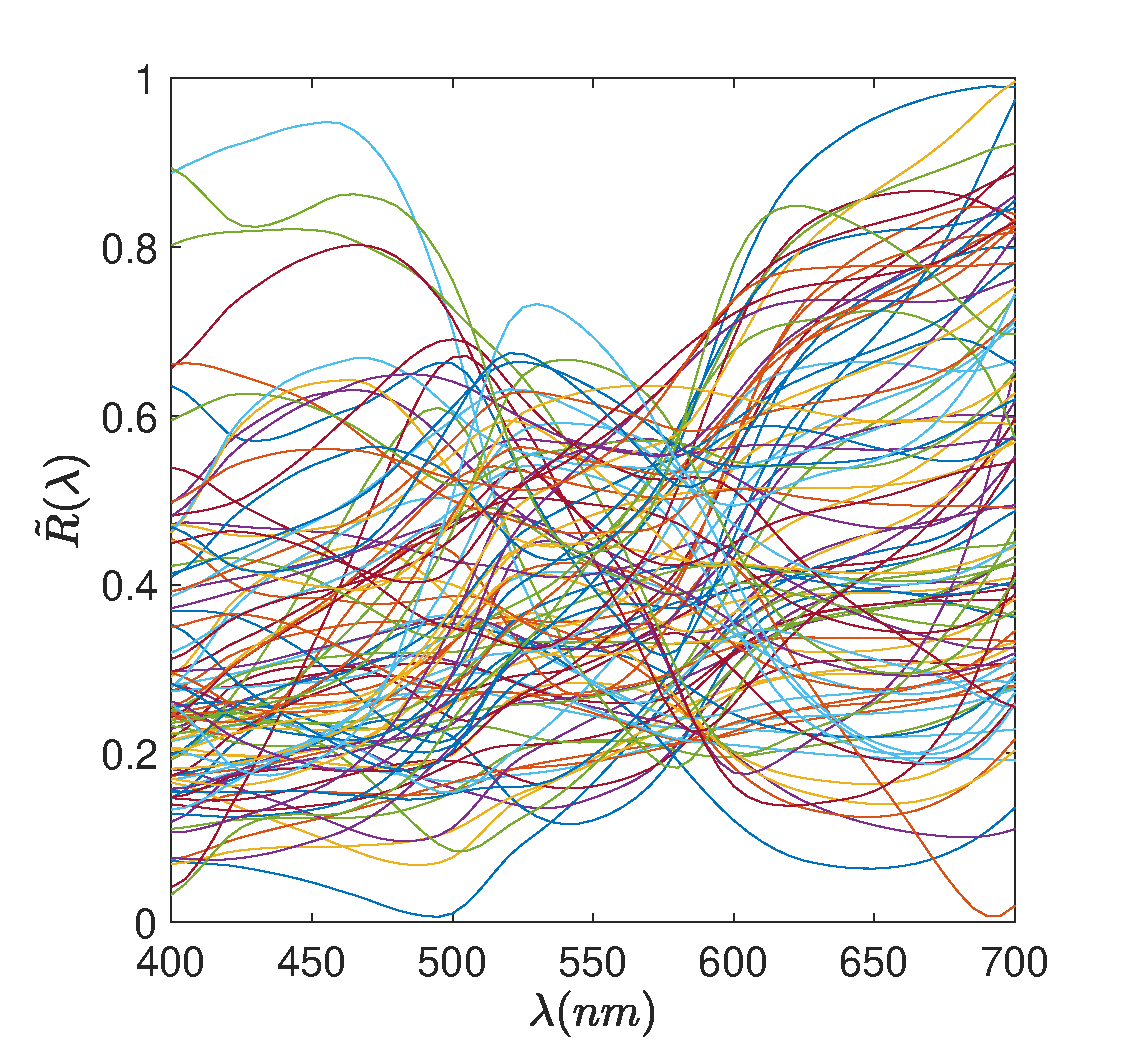
\includegraphics[width=\textwidth]{../Figures/Figure8/Figure8_b.pdf}
	\caption{SVD RF Performance}
	\label{fig:SVDBAR}
    \end{subfigure}
    ~ %add desired spacing between images, e. g. ~, \quad, \qquad, \hfill etc. 
    %(or a blank line to force the subfigure onto a new line)
        \begin{subfigure}[b]{0.3 \textwidth}
	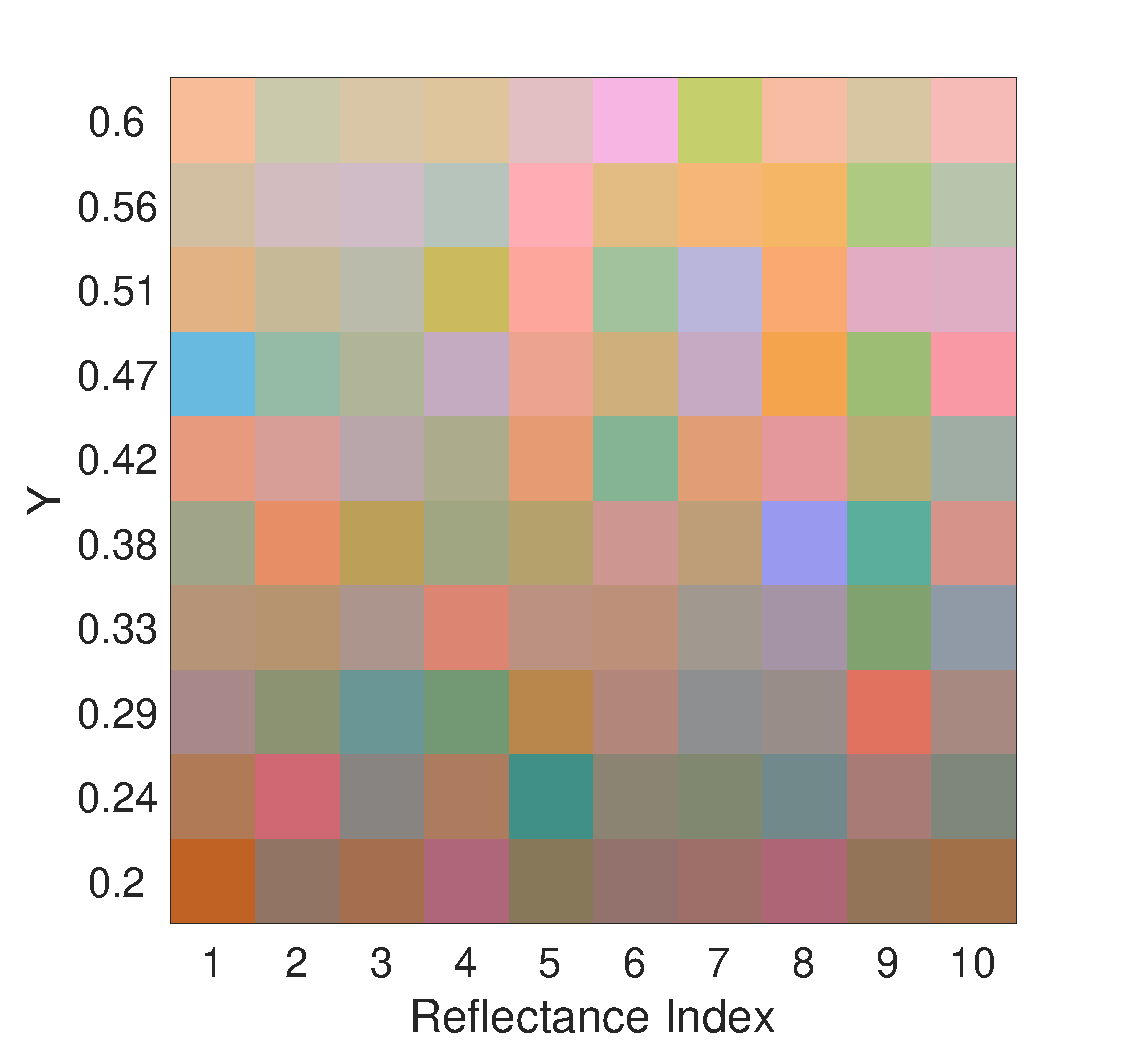
\includegraphics[width=\textwidth]{../Figures/Figure8/Figure8_c.pdf}
	\caption{AMA RF Performance}
	\label{fig:AMABAR}
    \end{subfigure}
\caption{{\bf Model and Filter Performance:} (a) Comparison of various methods on lightness estimations for the three cases studied here. For simple spectral variations, like where only the target reflectance varies (case 1) or only the target and illumination spectrum varies (Case 2), the lightness can be estimated well. This is so, because the lightness information can be estimated simply from the light reflected of the target( case 1) or from the contrast between the target and the {\it fixed} background (case 2). For more complex case, where the lightness information is confounded due to variations in target, background and illuminant (case 3), the estimation has higher variability. (b) Performance of the SVD receptive fields obtained from one case on the stimuli of others. The RFs obtained from any one of the three cases perform well on the stimuli from case 1. The RF of the most complicated case (case 3), has good performance on the stimuli of lower complexity. (c) Same as Fig.\ref{fig:SVDBAR} for AMA RFs.}
 \label{fig:barGraphs}
\end{figure}


\subsection{Lightness estimates and model performance}
Fig. ZZ gives the AMA lightness estimates for the three cases discussed above. We show the target object lightness estimates for there different methods: linear regression on center pixel, SVD regression and AMA. As is expected, when only the target object reflectance varies, it is easy to estimate the target object lightness. For case 2, where the light source spectra are allowed to vary, although the light captured by the cones vary from image to image, the contrast between the target and the background remains fixed and can be used to estimate the target object lightness. Thus, the SVD-LDA and AMA still provide good estimates of the target object lightness. In case 3, the most challenging case where all the spectra are allowed to change, AMA still does a reasonable job of estimating the target object lightness. AMA mean estimates lie close to the diagonal x=y line.

We compare the performance of these models using the relative root mean square estimator ($E_{\rm rel}$) defined as:

\begin{align}
E_{\rm rel} = \sqrt{\left\langle\left(\frac{Y_{\rm Est}-Y_{\rm Act}}{Y_{\rm Act}}\right)^2\right\rangle}
\end{align}

Fig. ZZZ shows $E_{\rm rel}$ for the various estimators used here.

\subsection{Explain the filters}

\section{Methods}
\subsection{Generating Virtual Images}
The light that reflects off an object and reaches our eyes depends on many factors. These factors include: the surface reflectance of the object, the surface reflectance, texture, material and geometry of the objects in its surround, the spectrum of the sources of light illuminating the object, and the position of the observer. In natural scenes, these spectral and geometrical factors vary considerably. To study the effect of these factors on color perception, we need a system that can generate natural scenes with precise control over all such factors. We need a system that can produce natural scenes at a fixed perceived color of a target object, while having a representative, but precisely quantified, sampling of the variations in the scene. Under natural conditions it is difficult to control and quantify every such parameter in a scene. Thus generating such a dataset, with a representative sampling of natural variations, is considerably time and labor intensive.

To overcome this  challenge, we have developed an image rendering software pipeline that allows us to specify a virtual, but naturalistic, statistical model of visual scenes with parametric control over factors in natural scenes. The software uses a physically-based image rendering system that accurately accounts for the interactions of light with matter in 3D scenes. It then renders a multi-spectral 2D image of each modeled visual scene. Wherever possible, we have incorporated statistical models of the variation of specific scene parameters based on observed data in natural scenes. In addition, our software simulates the responses of retinal cones to the rendered multi-spectral images using a realistic model of the early human visual system. Below we provide the details of the software and the choices made to generate ensembles of scenes with corresponding images. Our software, which is written in MATLAB, is freely available through a public respository: \href{https://github.com/BrainardLab/VirtualWorldColorConstancy}{Virtual World Color Constancy}. It builds on several other open source projects, including \href{http://rendertoolbox.org}{RenderToolbox4} \cite{heasly2014rendertoolbox3}, \href{http://isetbio.org}{Isetbio} and \href{https://www.mitsuba-renderer.org}{Mitsuba} \cite{jakob2015mitsuba}. Below we refer to the software pipeline as VWCC (for Virtual World Color Constancy).

The process of generating an individual virtual scene begins with the selection of a \textit{base scene} (Fig.~\ref{fig:baseScenes}). The base scene is a 3D model that defines a rendering space.  It typically includes the specification of a number of 3D objects and light sources, and is annotated with meta-data that may be used to guide the placement of additional objects and light sources, as well as the specification of camera position. VWCC includes a library of base scenes obtained from materials made available on the Internet under various Creative Commons licenses. We have found that there is sufficient variation in how nominally-standard graphics interchange file formats are used in practice that each base scene obtained from the Internet (which we refer to as \textit{wild scenes}) requires a certain amount of hand editing before it renders properly. We refer to this process, along with adding meta-data about the scene, as \textit{taming} a wild scene. Tame base scenes may also be created de novo using a 3D modeling software (e.g., \href{https://www.blender.org/}{Blender}).  The overall scale of the base scene may be adjusted under programmatic control or chosen randomly, adding to the available statistical richness. If one chooses to draw entries from the base scene library at random for each virtual scene, the base scene library then provides a simple statistical model of the gross layout of natural scenes. As time progresses, we plan to tame more wild scenes so as to increase the number of entries in the base scene library. Currently the library contains 6 base scenes: Library (Fig.~\ref{fig:baseSceneLibrary}), Mill (Fig.~\ref{fig:baseSceneMill}), Table-Chairs (Fig.~\ref{fig:baseSceneTableChairs}), Indoor plant (Fig.~\ref{fig:baseSceneIndoorPlant}), Checkerboard (Fig.~\ref{fig:baseSceneWarehouse}) and Warehouse (Fig.~\ref{fig:baseSceneCheckerBoard}).

% Figure 9
\begin{figure}[t]
\centering
\begin{subfigure}[b]{0.22 \textwidth}
        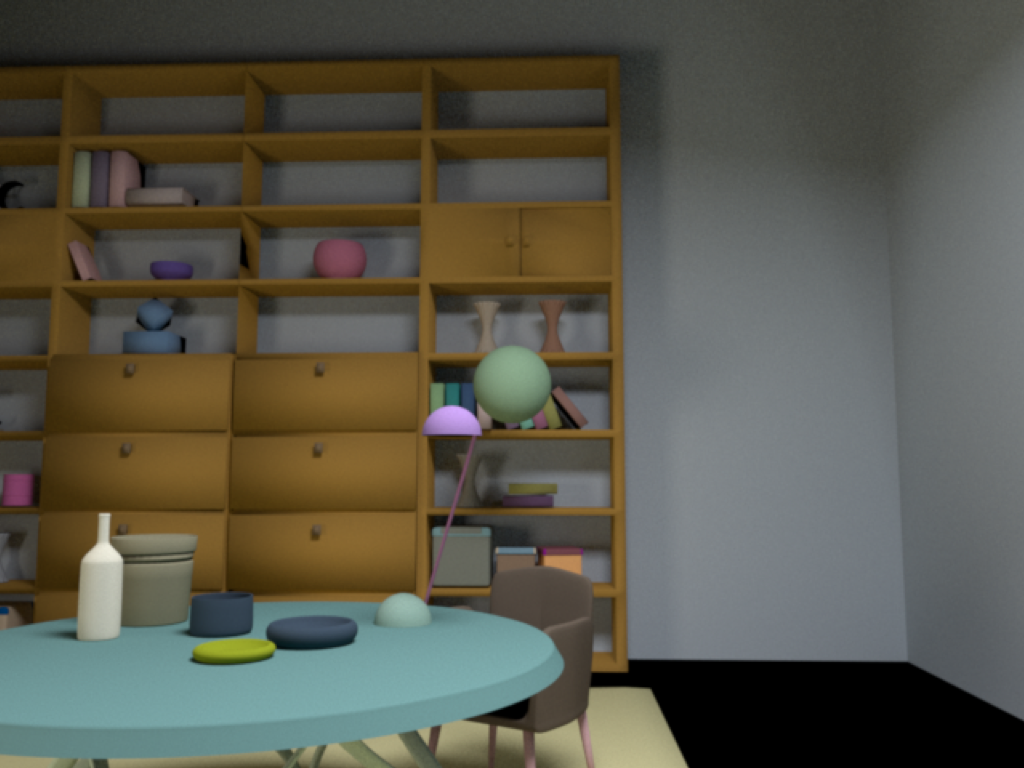
\includegraphics[width=\textwidth]{../Figures/Figure9/Figure9_a.png}
        \caption{Library }
        \label{fig:baseSceneLibrary}
    \end{subfigure}
    ~ %add desired spacing between images, e. g. ~, \quad, \qquad, \hfill etc. 
      %(or a blank line to force the subfigure onto a new line)
    \begin{subfigure}[b]{0.22 \textwidth}
        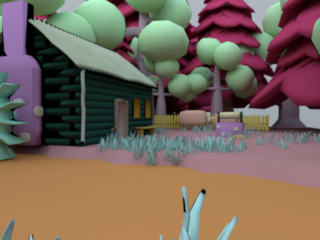
\includegraphics[width=\textwidth]{../Figures/Figure9/Figure9_b.png}
        \caption{Mill}
        \label{fig:baseSceneMill}
    \end{subfigure}    
    ~ %add desired spacing between images, e. g. ~, \quad, \qquad, \hfill etc. 
    %(or a blank line to force the subfigure onto a new line)
    \begin{subfigure}[b]{0.22 \textwidth}
        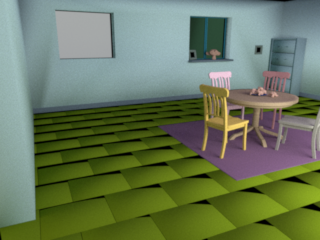
\includegraphics[width=\textwidth]{../Figures/Figure9/Figure9_c.png}
        \caption{Table-Chairs}
        \label{fig:baseSceneTableChairs}
    \end{subfigure}
    
    \begin{subfigure}[b]{0.22 \textwidth}
        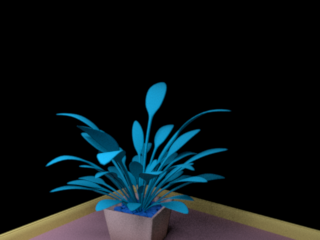
\includegraphics[width=\textwidth]{../Figures/Figure9/Figure9_d.png}
        \caption{Indoor-plant}
        \label{fig:baseSceneIndoorPlant}
    \end{subfigure}    
    ~
    \begin{subfigure}[b]{0.22 \textwidth}
        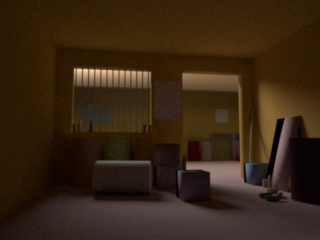
\includegraphics[width=\textwidth]{../Figures/Figure9/Figure9_e.png}
        \caption{Warehouse}
        \label{fig:baseSceneWarehouse}
    \end{subfigure}
    ~
    \begin{subfigure}[b]{0.22 \textwidth}
        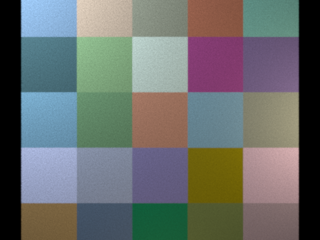
\includegraphics[width=\textwidth]{../Figures/Figure9/Figure9_f.png}
        \caption{Checkerboard}
        \label{fig:baseSceneCheckerBoard}
    \end{subfigure}
    \caption{Example of base scenes.}\label{fig:baseScenes}
\end{figure}

VWCC provides an option for inserting 3D objects and lights sources into the base scene. Fig.~\ref{fig:libraryWithTarget} shows examples of objects inserted in the library base scene. The object shapes may be selected from a VWCC library that, similar to the VWCC library of base scenes, has been tamed from materials made available on the Internet. The light sources may be chosen as point lights, area lights, or as shapes selected from the object library.

% Figure 10
\begin{figure}[h]
\centering
\begin{subfigure}[b]{0.22 \textwidth}
        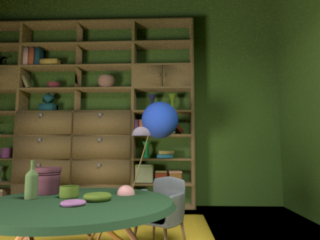
\includegraphics[width=\textwidth]{../Figures/Figure10/Figure10_a.png}
        \caption{Big-ball}
        \label{fig:libraryWithBigBall}
    \end{subfigure}
    ~ %add desired spacing between images, e. g. ~, \quad, \qquad, \hfill etc. 
      %(or a blank line to force the subfigure onto a new line)
\begin{subfigure}[b]{0.22 \textwidth}
        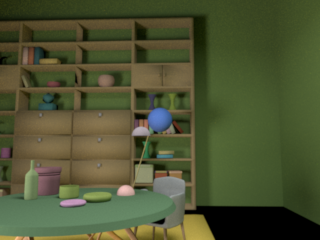
\includegraphics[width=\textwidth]{../Figures/Figure10/Figure10_b.png}
        \caption{Small-ball}
        \label{fig:libraryWithSmallBall}
    \end{subfigure}
    ~ %add desired spacing between images, e. g. ~, \quad, \qquad, \hfill etc. 
      %(or a blank line to force the subfigure onto a new line)
    \begin{subfigure}[b]{0.22 \textwidth}
        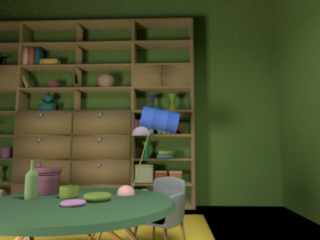
\includegraphics[width=\textwidth]{../Figures/Figure10/Figure10_c.png}
        \caption{Barrel}
        \label{fig:libraryWithBarrel}
    \end{subfigure}
    
    \begin{subfigure}[b]{0.22 \textwidth}
        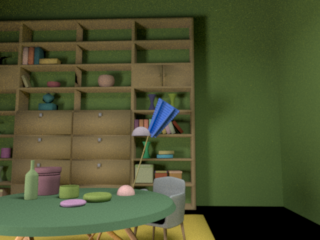
\includegraphics[width=\textwidth]{../Figures/Figure10/Figure10_d.png}
        \caption{Xylophone}
        \label{fig:libraryWithXylophone}
    \end{subfigure}
    ~
	\begin{subfigure}[b]{0.22 \textwidth}
        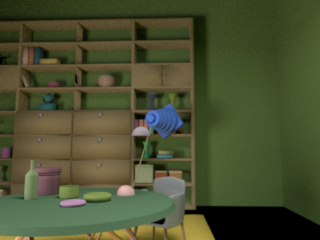
\includegraphics[width=\textwidth]{../Figures/Figure10/Figure10_e.png}
        \caption{Ring toy}
        \label{fig:libraryWithRingToy}
    \end{subfigure}
        ~
    	\begin{subfigure}[b]{0.22 \textwidth}
        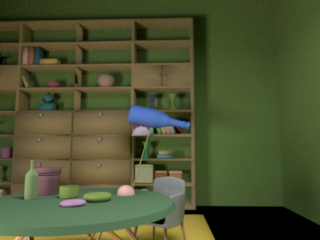
\includegraphics[width=\textwidth]{../Figures/Figure10/Figure10_f.png}
        \caption{Champagne Bottle}
        \label{fig:libraryWithChampagneBottle}
    \end{subfigure}
\caption{Base scenes with inserted objects.}\label{fig:libraryWithTarget}
\end{figure}

The size, position and orientation of the inserted objects and lights may be specified programatically (Fig.~\ref{fig:objectTransformations}) or chosen randomly under constraints provided by the base scene meta-data. As with the base scene library, the object may be drawn at random from the VWCC object library.  Thus, along with distributions that characterize parameters such as the number, size, shape and orientation of the inserted objects and light sources, we have a simple statistical model of the object and light source geometry of natural scenes. 

Once a base scene has been chosen and objects and light sources inserted, we assign spectral surface reflectance, texture, and material property to each object surface in the scene. We also assign the illuminant spectral power distribution to each light source in the scene. Objects in the VWCC library may contain more than one distinct surface, each of which may be assigned a different surface reflectance. As with object position, these may be specified programatically. In the present work, we use simple choices for texture (all surfaces spatially uniform) and material property (all surfaces matte) and focus on variation in surface spectral reflectance. 

[GOT TO HERE.  DHB.]
% Figure11
\begin{figure}
	\begin{subfigure}[b]{0.18 \textwidth}
    \centering
        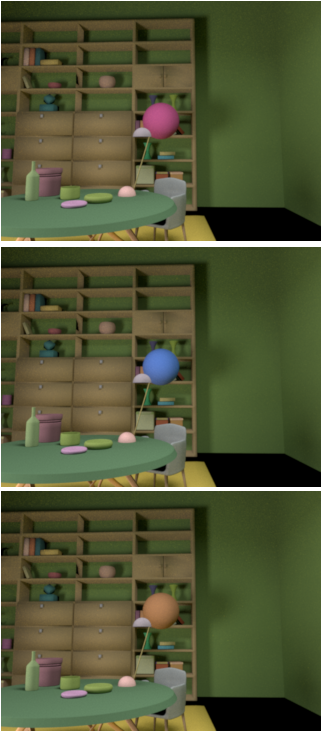
\includegraphics[width=\textwidth]{../Figures/Figure11/Figure11_a.png}
        \caption{Target spectra}
        \label{fig:targetVariation}
    \end{subfigure}
    ~ %add desired spacing between images, e. g. ~, \quad, \qquad, \hfill etc. 
      %(or a blank line to force the subfigure onto a new line)
    \begin{subfigure}[b]{0.18 \textwidth}
    \centering
        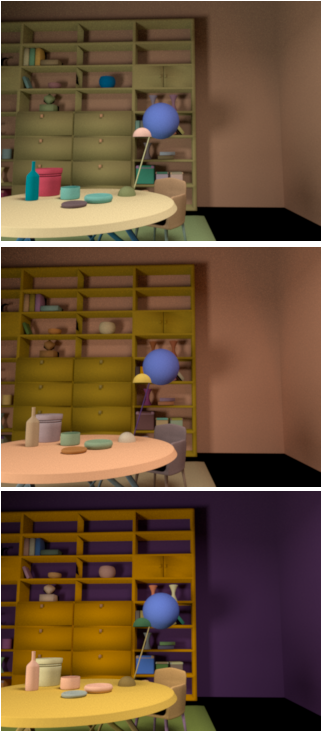
\includegraphics[width=\textwidth]{../Figures/Figure11/Figure11_b.png}
        \caption{Background spectra}
        \label{fig:backGroundVariation}
    \end{subfigure}
    ~ %add desired spacing between images, e. g. ~, \quad, \qquad, \hfill etc. 
    %(or a blank line to force the subfigure onto a new line)
    \begin{subfigure}[b]{0.18 \textwidth}
    \centering
        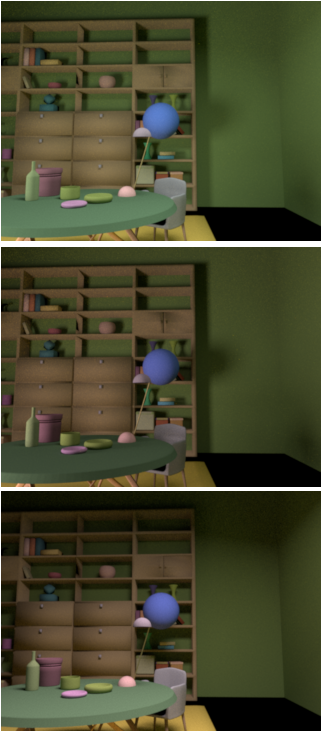
\includegraphics[width=\textwidth]{../Figures/Figure11/Figure11_c.png}
        \caption{Illumination spectra}
        \label{fig:illuminationVariation}
    \end{subfigure}
    ~ %add desired spacing between images, e. g. ~, \quad, \qquad, \hfill etc. 
      %(or a blank line to force the subfigure onto a new line)
	\begin{subfigure}[b]{0.18 \textwidth}
    \centering
        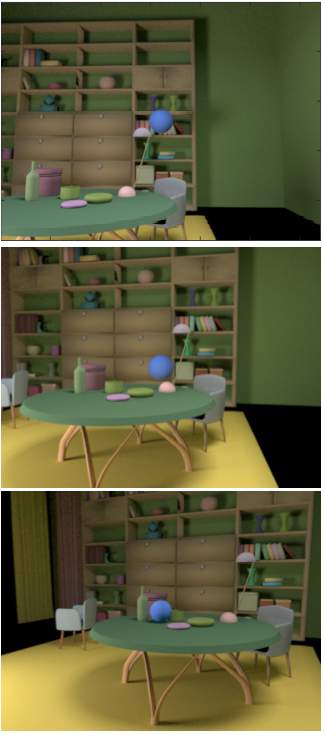
\includegraphics[width=\textwidth]{../Figures/Figure11/Figure11_d.png}
        \caption{Target position}
        \label{fig:targetPositionVariation}
    \end{subfigure}
    ~ %add desired spacing between images, e. g. ~, \quad, \qquad, \hfill etc. 
      %(or a blank line to force the subfigure onto a new line)
	\begin{subfigure}[b]{0.18 \textwidth}
    \centering
        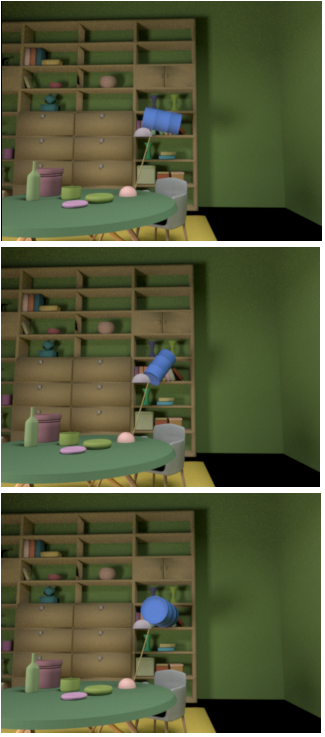
\includegraphics[width=\textwidth]{../Figures/Figure11/Figure11_e.png}
        \caption{Target Size/Orientation}
        \label{fig:targetSizeOrientation}
    \end{subfigure}
    ~ %add desired spacing between images, e. g. ~, \quad, \qquad, \hfill etc. 
      %(or a blank line to force the subfigure onto a new line)
    \caption{{\bf Transformations of the scene:} (a-c) Spectral Transformations. (d-e) Geometrical transformations.}\label{fig:spectralTransformations}
\end{figure}

After specifying the geometry and spectra, one of the inserted objects is chosen as the target object in the scene. A camera is inserted at a user specified position and then pointed at the target object. We ensure that the target object is not completely occluded by another object in the line of sight of the camera. Next, a predefined surface reflectance spectrum is assigned to the target object. This target surface reflectance sets the label for the virtual scene image. The scene is now rendered using the Mitsuba rendering package. The renderer produces 2D hyper-spectral images of the scene at specified wavelengths. Finally, these multi-spectral images are used to simulate retinal cone responses using the \href{https://github.com/isetbio}{ISETBIO} software.

To generate the retinal response one needs to specify the retinal cone mosaic and the size of the retinal image. The retinal cone mosaic is specified in terms of the total number of cones and the proportion of the long(L), medium(M) and the short(S) cones in the mosaic. With these parameters, the software generates the specified number of LMS cones with random positions on a square grid. The size of the retinal image is specified in terms of the field of view and object distance from the eye. 

For the images used in this work, we first selected the ``{\it Library}'' base scene from the VWCC base scene set. We inserted the spherical ``{\it Big Ball}'' object in the base scene and called it the target object. We also inserted a light source with the same spherical ``Big Ball'' shape. Also, a camera is inserted the scene and pointed at the target object. The position, and size of the inserted object, light source and the camera was held fixed for all the images analyzed in this work, i.e., no geometrical manipulations were performed between the images. Next, we assigned illumination and surface reflectance spectra to the lights and objects in the scene. The spectral manipulations for the various cases studied in this work are described below. Multi-spectral 2D images were rendered at 31 wavelengths from $400$nm to $700$nm spaced $10$nm apart at an image size $320\times 240$ pixel$^2$. Next, a $51 \times 51$ pixel$^2$ patch of the multi-spectral image was cropped around the target object and cone responses were calculated to these cropped images as described below.

\subsection{Illumination Spectrum}
The illumination spectrum is generated through a random statistical sampling of a natural illumination spectrum dataset. First, we decompose the spectra in the database as a linear sum using principle component analysis (PCA) basis vectors. This decomposition is approximated by taking a sum over the PCA basis vectors corresponding to the largest 6 eigenvalues. Random spectra are sampled from this low 6 dimensional PCA space assuming the spectral distribution to be a multivariate gaussian.

% Figure 12
\begin{figure}
\centering
	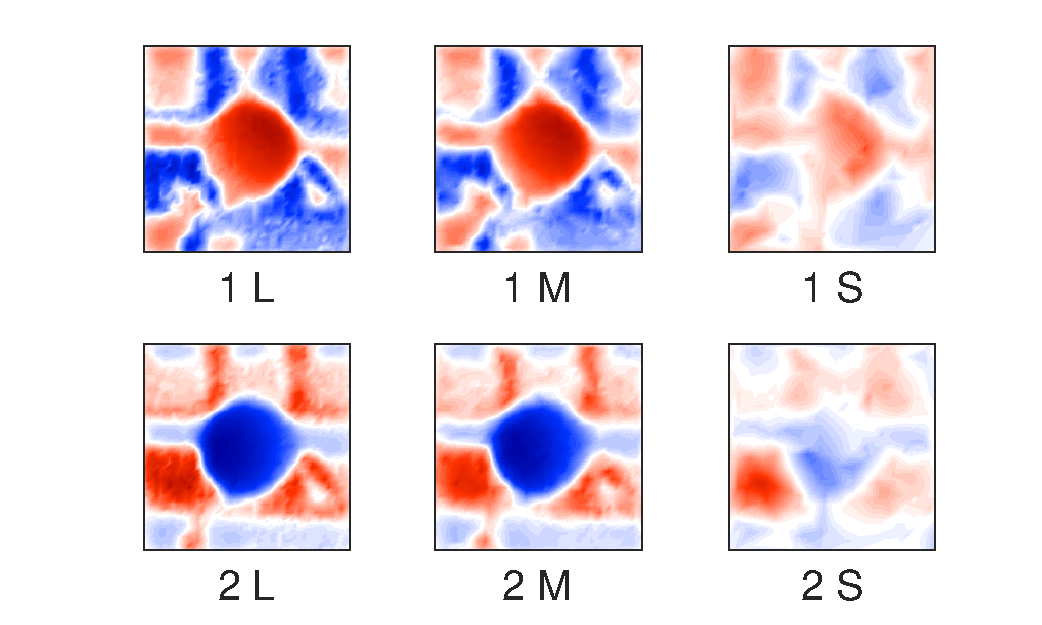
\includegraphics[width=\textwidth]{../Figures/Figure12/Figure12.pdf}
    \caption{Illumination Generation}
    \label{fig:illuminationGeneration}
\end{figure}
We have used the Granada natural daylight spectrum \href{http://colorimaginglab.ugr.es/pages/Data}{dataset} \cite{peyvandi2016colorimetric} to sample illuminants. Let us denote the Granada dataset as $I^G_i(\lambda)$, where $\{i \in [1,M]\}$ and $M$ is the total number of spectra in the dataset. Since the distribution varies over multiple order of magnitudes, we rescale each spectrum by dividing by its mean $I_i^s(\lambda) = \frac{I^G_i(\lambda)}{\int d\lambda I^G_i(\lambda)}$. These rescaled spectra $(I_i^s(\lambda))$ are then mean centered for PCA by subtracting out the mean 
rescaled spectra, $\bar{I}^{s}(\lambda) = \frac{1}{M}\sum_i{I_i^s(\lambda)}$. 
The resulting dataset, $I_i^{MC}(\lambda) = I_{s}(\lambda) - \bar{I}_{s}(\lambda)$, 
is decomposed as $I_i^{MC}(\lambda) = \sum_j w_{ij}\hat{{\bf e}}_j^{PCA}$, 
where $\hat{{\bf e}}_j^{PCA}$s are PCA basis vectors obtained using 
singular value decomposition (SVD). $w_{ij}$s are the projections 
of $I_i^{MC}(\lambda)$ along the PCA basis vectors. We approximate 
this decomposition by summing over the basis vectors corresponding to
the largest six SVD eigenvalues. For the Granada dataset, these six 
eigenvalues constitute more than $98\%$ of the variance. These steps
can be summarized as follows:
\begin{align}
I^G_i(\lambda) \rightarrow I_i^s(\lambda) = \frac{I^G_i(\lambda)}{\int d\lambda I^G_i(\lambda)} \rightarrow I_i^{MC}(\lambda) = I_{s}(\lambda) - \bar{I}_{s}(\lambda) \rightarrow I_i^{MC}(\lambda) = \sum_j w_{ij}\hat{{\bf e}}_j^{PCA}
\end{align}

To generate new illuminants $\tilde{I}_i(\lambda)$, random 
projection weights ($\tilde{w}_{ij}$) are generated using a multivariate 
gaussian distribution with mean $\bar{w}_j = \frac{1}{M}\sum_i w_{ij}$, 
and co-variance $\Sigma_{jj'} = \frac{1}{M} \sum_i \left(w_{ij} -\bar{w}_j\right)\left(w_{ij'} -\bar{w}_{j'}\right) $. If the $\tilde{w}_{ij}$ are such that, $\left( \sum_j \tilde{w}_{ij} \hat{{\bf e}}_j^{PCA} +  \bar{I}_{s} (\lambda)\right) > 0$, for all $\lambda$, then the new illuminant spectrum is given as 
\begin{align}
\tilde{I}(\lambda) = \left( \tilde{I}_{MC}(\lambda) + \bar{I}_{s}(\lambda)\right) 
\times \max\left(\langle I_{G}\rangle\right) .
\end{align}
Finally $\tilde{I}(\lambda)$ is rescaled by a uniform random number between [0, 300].

% Figure 13
\subsection{Reflectance Spectrum}
\begin{figure}
\centering
	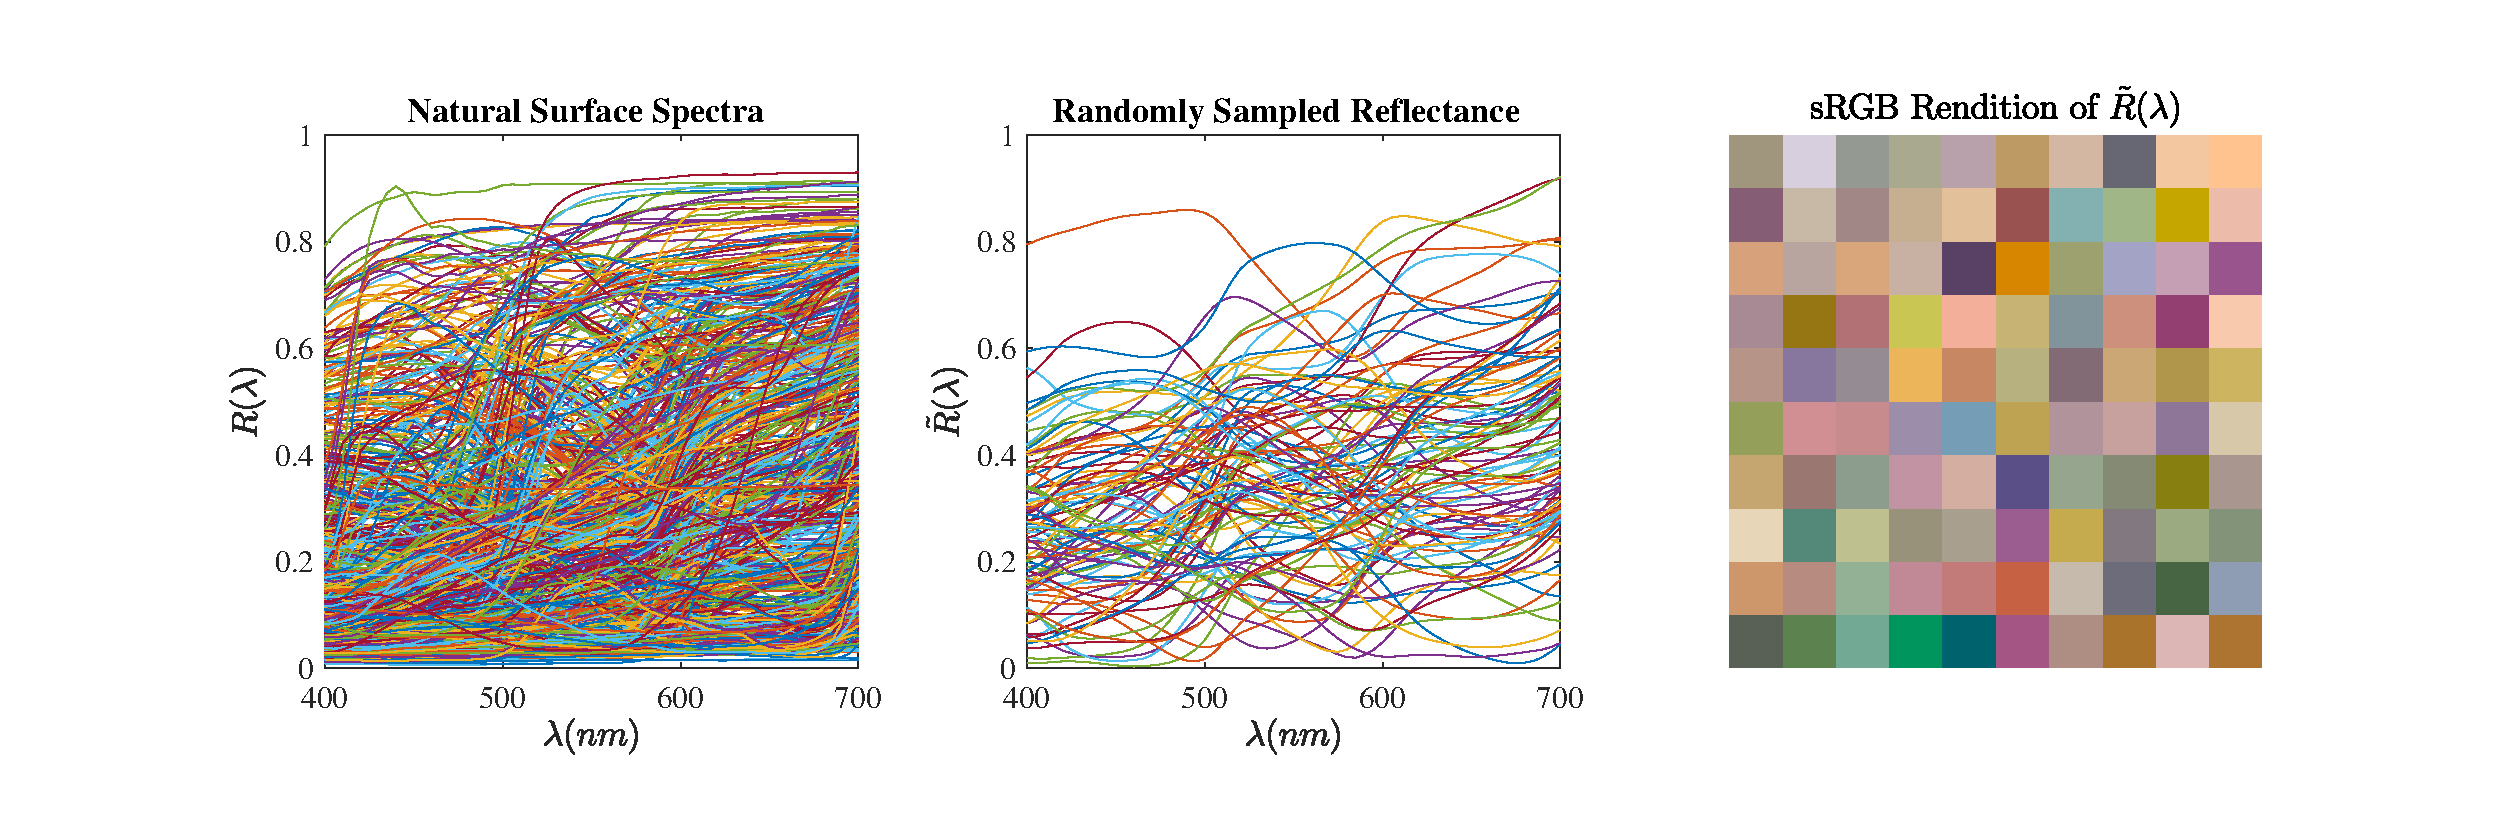
\includegraphics[width=\textwidth]{../Figures/Figure13/Figure13.pdf}
    \caption{Reflectance Generation}
    \label{fig:reflectanceGeneration}
\end{figure}

Similar to the illumination spectrum, the reflectance spectrum of the 
objects in the visual scene are generated through a random 
sampling of natural surface reflectance spectra. We have used 
the Munsell {(\it citation)} and vrhel {(\it citation)} surface reflectance 
datasets for such sampling. Let us denote the dataset of natural 
reflectance spectra as $R_i(\lambda)$, where $\{i \in [1,M]\}$ 
and $M$ is the total number of spectra in the dataset. To generate 
a random reflectance spectrum $\tilde{R}(\lambda)$, 
we first mean center the dataset by subtracting out the 
mean surface reflectance spectrum, $\bar{R}(\lambda)$,
from each surface reflectance spectrum.
$\bar{R}(\lambda)$ is obtained by taking the sample 
mean over all spectra in the dataset, i.e.,
$\bar{R}(\lambda) = \frac{1}{M} \sum_{i=1}^M R_i(\lambda)$. 
Thus we have the mean centered reflectance 
spectrum dataset as $R_i^{\rm MC}(\lambda) =  R_i(\lambda)-\bar{R}(\lambda)$. 
We decompose this as $R_i^{\rm MC}(\lambda) = \sum_j{w_{ij} \; {\bf \hat{e}}_j^{\rm PCA}}$. Here,
${\bf \hat{e}}_j^{\rm PCA}$s are PCA basis vectors obtained using SVD 
and $w_{ij}$s are the projections of $R_i^{\rm MC}(\lambda)$ along the PCA eigenvectors 
$\left( w_{ij} = R_i^{\rm MC}(\lambda)\cdot {\bf \hat{e}}_j^{\rm PCA}\right)$. The 
decomposition is approximated by summing over the PCA basis 
vectors corresponding to the largest six SVD eigenvalues. These six eigenvalues capture 
more than $92\%$ of the variance in the combined Munsell and vhrel datasets. To generate 
a new reflectance spectrum, a point is sampled randomly in this 
six dimensional sub-space using a multivariate normal 
distribution, with mean $\bar{w}_j = \frac{1}{M}\sum_i w_{ij}$, 
and co-variance $\Sigma_{jj'} = \frac{1}{M} \sum_i \left(w_{ij} -\bar{w}_j\right)\left(w_{ij'} -\bar{w}_{j'}\right) $. If the randomly sampled projection, $\tilde{w}_{ij}$, is 
such that $\left( 0 < \sum_j \tilde{w}_{ij}{\bf \hat{e}}_j^{\rm PCA} + \bar{R}(\lambda)<1\right) $ at every $\lambda$, the new surface reflectance 
is given as: $\tilde{R}_i(\lambda) =\sum_j \tilde{w}_{ij}{\bf \hat{e}}_j^{\rm PCA} + \bar{R}(\lambda)$.

% Figure 14
\begin{figure}
\centering
	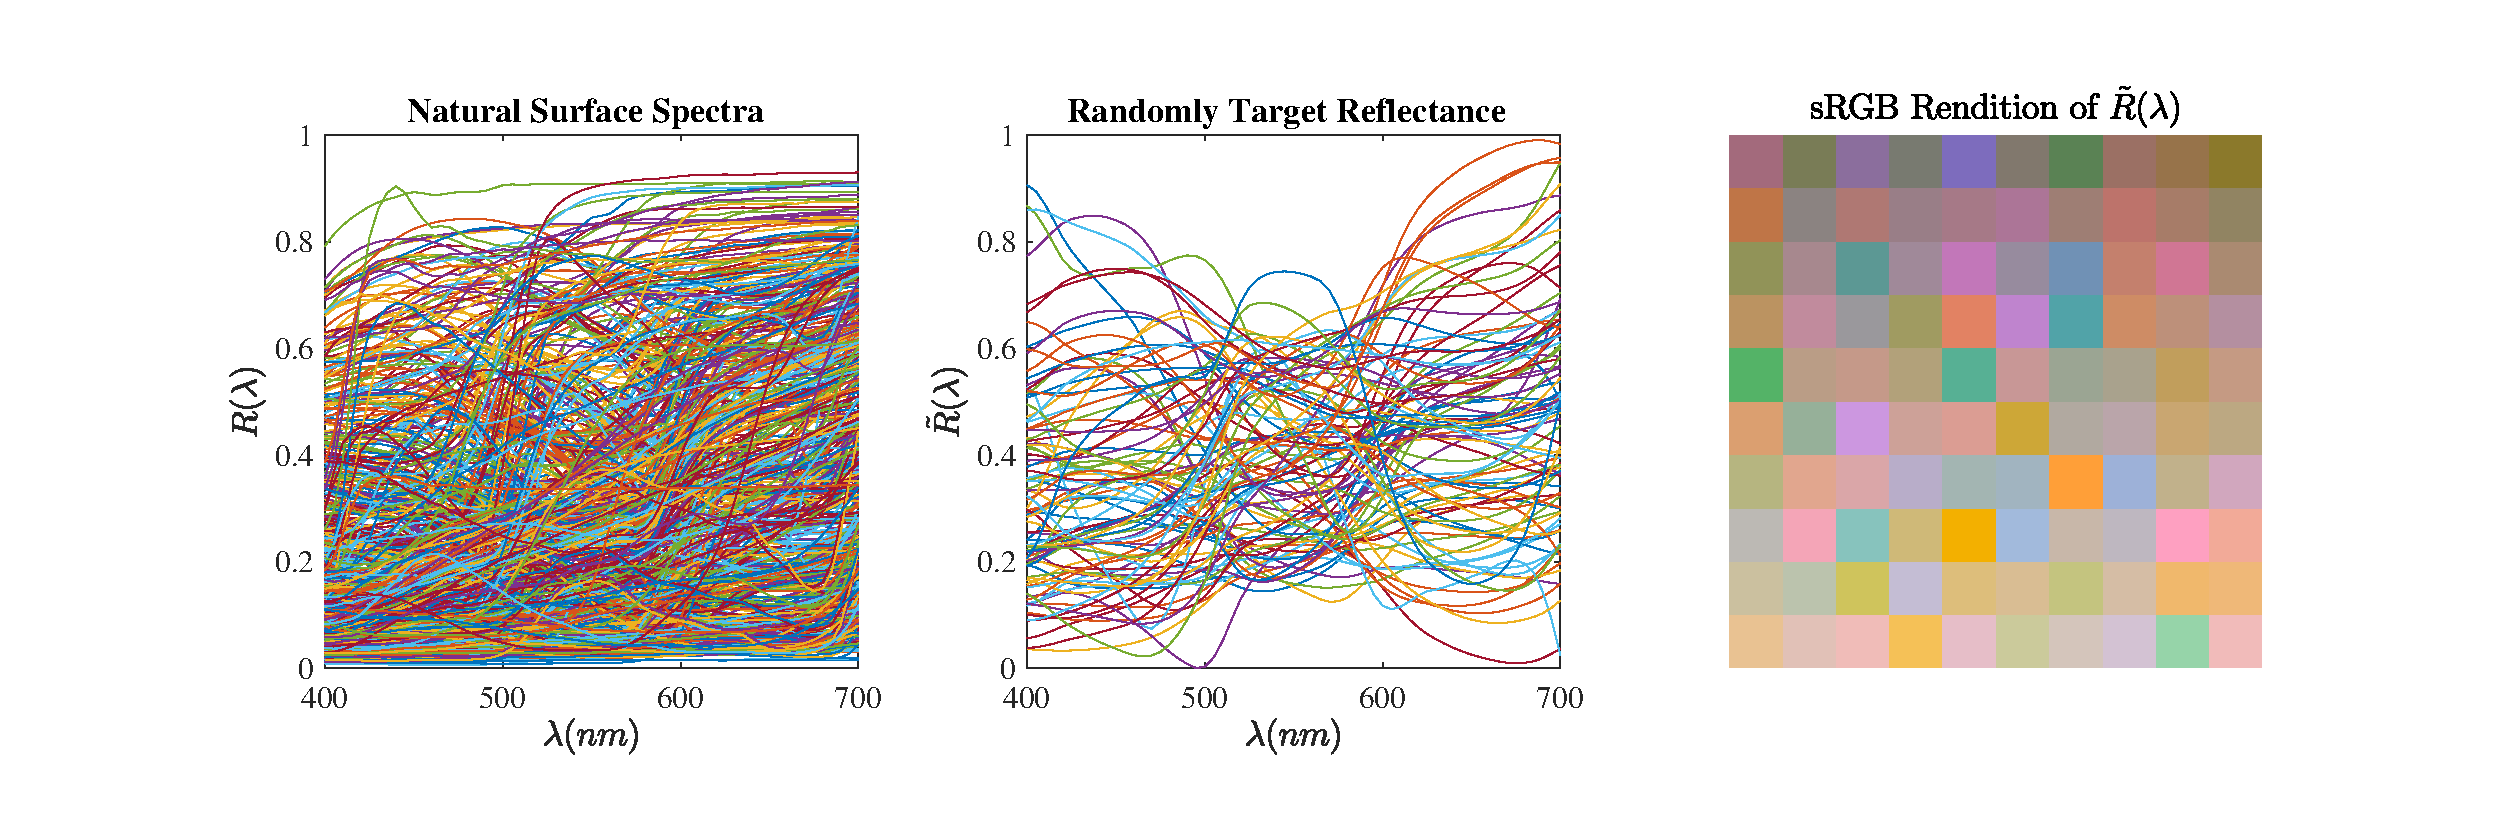
\includegraphics[width=\textwidth]{../Figures/Figure14/Figure14.pdf}
    \caption{Target Reflectance Generation}
    \label{fig:targetGeneration}
\end{figure}

For generating the target object reflectance at a particular lightness $(Y_{\rm T})$, the values in the spectrum are 
rescaled by a scalar such that the perceived lightness of the 
target surface under standard daylight illuminant $(D_{65}(\lambda))$ 
equals a designated value. The scaling equals $\frac{Y_{\rm T}}{\int d\lambda \tilde{R}(\lambda) D_{65}(\lambda) \bar{y}(\lambda)}$, with $\bar{y}(\lambda)$ being the CIE luminosity (or luminous efficiency) function. 
$\bar{y}(\lambda)$ describes the average spectral sensitivity of human visual 
perception of brightness. The target reflectance is given by: $\tilde{R}(\lambda) \cdot\left(\frac{Y}{\int d\lambda \tilde{R}(\lambda) D_{65}(\lambda) \bar{y}(\lambda)}\right)$.

\subsection{Cone response to hyper-spectral images}
Cone response to the hyper-spectral images are generated
using \href{https://github.com/isetbio}{ISETBIO}. The model incorporates several critical components of biological vision, including physiological optics, information about cornea, lens, pupil, etc. We simulate a model retinal mosaic with $51\times51$ cones having cone densities in the ratio [l,m,s]=[0.6 0.3 0.1]. The cone wavelength sensitivities are scaled such that the area under the sensitivity curve equals unity. A $51\times51$ pixel$^2$ patch of the image containing the target image is used to calculate the cone responses. The image patch is assumed to cover a $1^{\circ}$ field of view at a distance of 1 m. 

\subsection{Accuracy Maximization Analysis}
AMA \cite{geisler2009optimal,burge2017accuracy} is a Bayesian ideal observer model for task specific dimensionality reduction. It finds the receptive fields that are optimal for performing a well defined behavioral task. Given a labeled training set, a noisy response model, and a cost function, AMA returns a set of linear receptive fields that are optimal for performing a task, which is implicitly defined in terms of the labels. The optimal filters are the ones whose noisy response to the stimuli, as given by the specified response model, minimizes the cost function over the training set. The filters are learned via gradient descent with the aid of an optimal Bayesian decoder that is matched to the filters throughout the learning process. 

Let us assume that there is a latent variable ($X$) that takes the values $\{X_k: k\in[1,N_{\nu}] \}$. The $l$'th stimuli corresponding to the the $k$'th category of the latent variable is $s_{kl}$. Let us assume that there is a set of linear filters {\textbf{\textit f}} which when acting on $s_{kl}$ gives the response ${\textbf{\textit R}}_{kl}$. Let's say we have a decoder $g$ that takes ${\textbf{\textit R}}_{kl}$ as the input and returns an estimate of the latent variable ($X_k$) corresponding to the stimuli $s_{kl}$ as $\hat{X}_{kl}$. Given this estimate, one can define a cost function $C_{kl}(X_{kl},\hat{X}_{kl})$ corresponding to specific response ${\textbf{\textit R}}_{kl}$ and a mean cost $\bar{C}_{kl}(X_{kl},\hat{X}_{kl})$ corresponding to the average response $r_{kl} = \langle{\textbf{\textit R}}_{kl}\rangle$. 

Accuracy maximization analysis (AMA) finds the set of optimal filters ${\textbf{\textit f}}^{\rm opt}$ that minimize the average cost function over the entire dataset $\{s_{kl}: k\in[1,N_{\nu}, l\in[1,N_k]\}$. $N_{\nu}$ is the total number of labels and $N_{k}$ is the number of stimuli corresponding to the label $X_k$. Thus,
\begin{align}
{\textbf {\textit f} }^{\rm opt} = \argmin_{\textbf {\textit f} } \sum_{kl} \bar{C}_{kl}.
\label{eq:fopt}
\end{align}

AMA employs the Bayes optimal decoder to estimate the optimal estimate. The Bayesian decoder computes the posterior probability of the latent variable $p(X|{\textbf {\textit R}})$ and reads out the optimal estimate $\hat{X}^{\rm opt}$ from the posterior as the value that minimizes the cost. By Bayes' theorem, the posterior probability can be written as:
\begin{align}
p(X_k|{\textbf {\textit R} }_{kl}) = \frac{p({\textbf {\textit R} }_{kl}|X_k)p(X_k)}{\sum\limits_{i=1}^{N_{\nu}}{p({\textbf {\textit R} }_{kl}|X_i)p(X_i)}}.
\label{eq:posterior}
\end{align}
As conditional probability of the filter response is:
\begin{align}
p({\textbf {\textit R} }_{kl}|X_k) = \sum\limits_{m=1}^{N_k}p({\textbf {\textit R} }_{kl}|{\textbf {\textit s} }_{km})p({\textbf {\textit s} }_{km}|X_k),
\label{eq:condProb}
\end{align}
using Eq.\ref{eq:condProb} in Eq.\ref{eq:posterior} we get:
\begin{align}
p(X_k|{\textbf {\textit R} }_{kl}) = \frac{\left[\sum\limits_{m=1}^{N_k}p({\textbf {\textit R} }_{kl}|{\textbf {\textit s} }_{km})p({\textbf {\textit s} }_{km}|X_k)\right]p(X_k)}{\sum\limits_{i=1}^{N_{\nu}}{\left[\sum\limits_{j=1}^{N_j}p({\textbf {\textit R} }_{il}|{\textbf {\textit s} }_{ij})p({\textbf {\textit s} }_{kj}|X_i)\right]p(X_i)}}
\label{eq:finalPosterior}
\end{align}
Since, $p({\textbf {\textit s} }_{km}|X_k) = \frac{1}{N_k}$, and $p(X_k)=\frac{N_k}{N}$, where $N = \sum\limits_{k=1}^{N_{\nu}}N_{k}$ is total number of samples in the training set, Eq.\ref{eq:finalPosterior} simplifies to
\begin{align}
p(X_k|{\textbf {\textit R} }_{kl}) = \frac{\left[\sum\limits_{m=1}^{N_k}p({\textbf {\textit R} }_{kl}|{\textbf {\textit s} }_{km}) \frac{1}{N_k}\right]\frac{N_k}{N}}{\sum\limits_{i=1}^{N_{\nu}}{\left[\sum\limits_{j=1}^{N_j}p({\textbf {\textit R} }_{il}|{\textbf {\textit s} }_{ij}) \frac{1}{N_i}\right]\frac{N_i}{N}}} = \frac{\sum\limits_{m=1}^{N_k}p({\textbf {\textit R} }_{kl}|{\textbf {\textit s} }_{km})}{\sum\limits_{i=1}^{N_{\nu}}{\sum\limits_{j=1}^{N_j}p({\textbf {\textit R} }_{il}|{\textbf {\textit s} }_{ij})}}.
\label{eq:simplifiedPosterior}
\end{align}
Now if the cost associated with the latent variable $X_k$ and the estimate $\hat{X}_k$ is $\gamma (X_k,\hat{X}_k)$, we have  
\begin{align}
C_{kl} = \sum\limits_{u=1}^{N_{\nu}}\gamma(X_u,\hat{X}_u)p(X_u|{\textbf{\textit R}}_{kl}),
\end{align}
and the total cost associated with the training set is $\bar{C} = \frac{1}{N} \sum\limits_{k,l}\bar{C}_{kl} = \frac{1}{N} \sum\limits_{k,l}\langle C_{kl}\rangle_{{\textbf{\textit R}}_{kl}}$. The optimal AMA filters are obtained by minimizing $\bar{C}$ over the filter set ${\textbf {\textit f} }$ (Eq.\ref{eq:fopt}). The filters are obtained using gradient descent.

In this work, we assume the noisy response model to be a multivariate gaussian. For a stimuli $s_{kl}$, the noisy response vector ${\textbf{\textit R}}_{kl} = \left[{\textbf{\textit R}}_{kl,1},{\textbf{\textit R}}_{kl,2},\dots,{\textbf{\textit R}}_{kl,q}\right]$ to the set of filters ${\textbf{\textit f}} = \left[{\textbf{\textit f}}_{kl,1},{\textbf{\textit f}}_{2},\dots,{\textbf{\textit f}}_{q}\right]$ is given by $\mathcal{N}({\textbf{\textit r}}_{kl}, \Sigma)$, with mean response vector ${\textbf{\textit r}}_{kl} = \left[{\textbf{\textit r}}_{kl,1},{\textbf{\textit r}}_{kl,2},\dots,{\textbf{\textit r}}_{kl,q}\right] = \left[{\textbf{\textit f}}_{1}\cdot s_{kl},{\textbf{\textit f}}_{2}\cdot s_{kl}\dots,{\textbf{\textit f}}_{q}\cdot s_{kl}\right]$ and the covariance matrix as the diagonal matrix $\Sigma$ with variances $\left(\sigma_1^2, \sigma_2^2,\dots, \sigma_q^2 \right)$. We assume $\sigma_i^2 = \alpha |r_i| + \sigma_0^2$, $|{\textbf{\textit f}}_{kl,i}|=1$ and $s_{kl}$ to be zero mean contrast normalized, i.e., $\langle{s_{kl}}\rangle = 0$ \& ${|s_{kl}|=1}$.

\subsection{Data Analysis} We generate XX number of images with target objects at 10 standard luminance levels linearly spaced between 0.2 to 0.6. These limits were chosen because the luminance under the standard source ($D_{65}$) of more than $90\%$ of the natural surface reflectance spectra fell between them. Thus we had YY images at each target luminance level. We generated the cone responses to these images using ISETBIO. The cone response ($I$) were first converted in to weber contrast form using the transformation $\left(I \rightarrow I_{\rm web} = \frac{I}{\langle I \rangle}-1\right)$. The weber contrast responses and the target luminance levels were used as the input stimuli and the latent variable, respectively, for AMA. The AMA parameters were: $\alpha = xxx$ and $\sigma_0^2 = yyy$.


\subsection{Explanation of the various cases}
In this work we have labeled the images using the lightness of the target object under  standard daylight spectrum ($D_65$). The images are labeled such that the total light reflected from the target object equals a fixed value. At this fixed value, we generate multiple images with variations in the spectral properties of the objects and the light sources. At fixed target lightness (Y65), spectral variations can result from variations in the shape of: 1. Target surface reflectance spectrum, 2. Background object surface reflectance, and 3. Spectral power distribution of the light source. These give rise to 12 distinct cases (Fig. \ref{fig:caseIcons}). The icons on the left and the top represent the spectrum of the illuminant, the background and the target object. For the illuminant and background, only one curve in the represents fixed spectra from image to image. Two curve imply that the spectra were varied randomly from image to image. For the target object, we show the spectrum at two distinct lightness levels. At a particular level, the meaning of the curves is the same as that of illuminant and background icons. Additionally, same shape of the target reflectance spectrum at both the levels means that Y65 was changed by changing the mean value of the surface reflectance spectrum keeping the same shape.

%\begin{figure}
%\centering
%	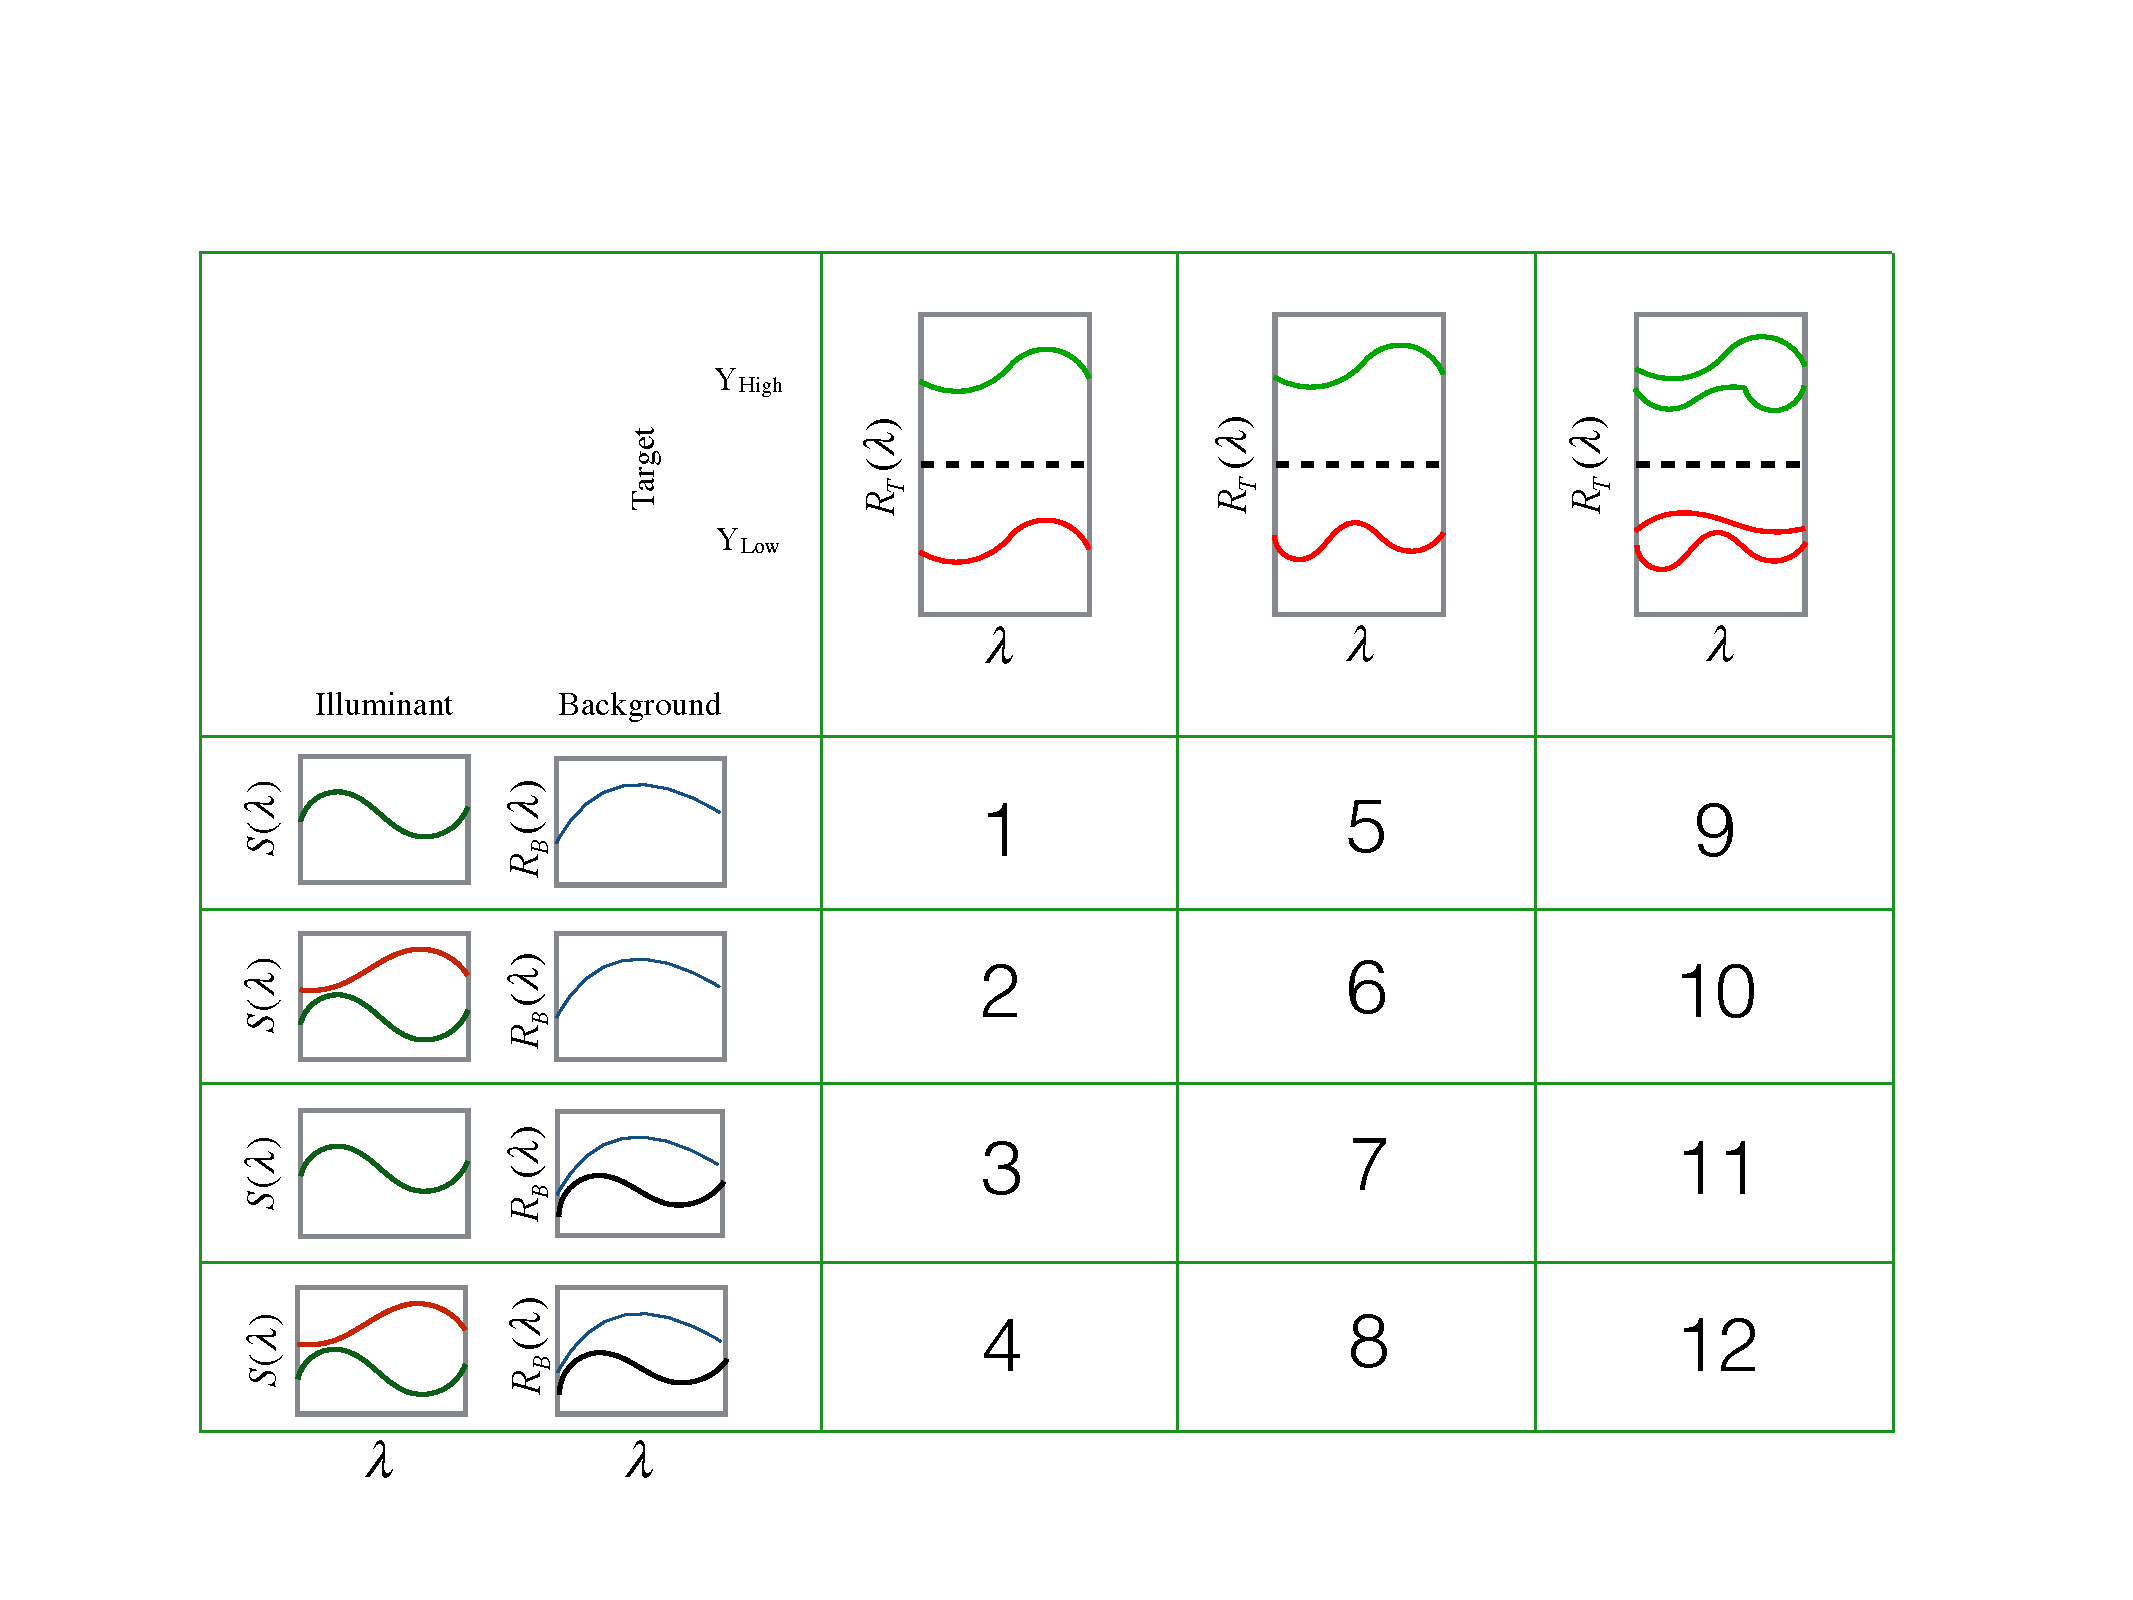
\includegraphics[width=0.6 \textwidth]{cases.pdf}
%    \caption{\bf{Spectral variations considered in our analysis.} }
%    \label{fig:casesIcons}
% \end{figure}

To illustrate, in case 1 the spectral power distribution of the light source and the surface reflectance of the background objects are fixed from image to image. Further, the shape of the target object surface reflectance also remains the same from to image to image at the same standard lightness level, and only vary in their mean value between standard luminance levels. Thus in case 1, at one standard lightness, all images are identical (Fig. . This is the simplest possible scene variation considered here. Similarly, in the most complex case, case 12, all the spectra are allowed to vary from image to image. 



\bibliography{references}
\bibliographystyle{jovcite}

\end{document}

